% !TEX program = pdflatex
% Collaboration talk (English) — Muon azimuthal asymmetry with the UMD and the SD
% Lautaro Silva Pizzi — ITeDA (CNEA-CONICET-UNSAM) / FCEN-UBA — short version (12 min) for the
% Auger Collaboration Meeting (19 November 2026), from the UMD Foundations Meeting deck
% (charla_colaboracion_2026.tex)
% Template: claude_work/presentacion_defensa_2026 (metropolis + ITeDA palette).
% Content and numbers: thesis Ch. 5 and 6; see borrador_charla.md for sources and open points.
% Build: ./compilar.sh  ->  charla_colaboracion_2026.pdf (slides) and
%                            charla_colaboracion_2026_notas.pdf (slides + speaker notes).
\documentclass[aspectratio=169,11pt]{beamer}

\usetheme{metropolis}
\usepackage[utf8]{inputenc}
\usepackage[T1]{fontenc}
\usepackage[english]{babel}
\usepackage{lmodern}
\renewcommand{\familydefault}{\sfdefault}
\usepackage{amsmath,amssymb}
\usepackage{graphicx}
\usepackage{booktabs}
\usepackage{tikz}
\usetikzlibrary{arrows.meta, positioning, calc, shapes.geometric}
\usepackage{appendixnumberbeamer}
\graphicspath{{figuras/}}

\ifdefined\withnotes
  \setbeameroption{show notes}
\fi
\setbeamertemplate{note page}[plain]
\setbeamerfont{note page}{size=\small}

% Paleta ITeDA (muestreada del logo institucional) y ajustes de color sobre metropolis.
\definecolor{itedaTeal}{HTML}{1B5E7E}
\definecolor{itedaTealDark}{HTML}{123847}
\definecolor{itedaOrange}{HTML}{F07E26}
\definecolor{itedaLight}{HTML}{F5F7F8}
\definecolor{itedaGray}{HTML}{5A6B72}

\setbeamercolor{palette primary}{bg=itedaTeal, fg=white}
\setbeamercolor{palette secondary}{bg=itedaTealDark, fg=white}
\setbeamercolor{palette tertiary}{bg=itedaTealDark, fg=white}
\setbeamercolor{title separator}{fg=itedaOrange}
\setbeamercolor{progress bar}{fg=itedaOrange, bg=itedaTeal!25}
\setbeamercolor{progress bar in head/foot}{fg=itedaOrange, bg=itedaTeal!35}
\setbeamercolor{frametitle}{bg=itedaTeal, fg=white}
\setbeamercolor{normal text}{fg=itedaTealDark}
\setbeamercolor{alerted text}{fg=itedaOrange}
\setbeamercolor{example text}{fg=itedaTeal}
\setbeamercolor{background canvas}{bg=white}
\setbeamercolor{itemize item}{fg=itedaOrange}
\setbeamercolor{itemize subitem}{fg=itedaTeal}
\setbeamercolor{block title}{bg=itedaTeal, fg=white}
\setbeamercolor{block body}{bg=itedaLight, fg=itedaTealDark}
\setbeamercolor{block title alerted}{bg=itedaOrange, fg=white}
\setbeamercolor{block body alerted}{bg=itedaOrange!12, fg=itedaTealDark}

% Colores que replican las trazas de la Fig. "Componentes del SD: EM & Muónica vs. UMD"
\definecolor{plotBlue}{HTML}{1414B4}
\definecolor{plotGreen}{HTML}{2E8B57}
\definecolor{plotMaroon}{HTML}{8B1A1A}


\setbeamertemplate{navigation symbols}{}
\setbeamertemplate{frame numbering}[fraction]
\setbeamerfont{footnote}{size=\tiny}
\setbeamerfont{itemize/enumerate body}{size=\small}
\setbeamerfont{itemize/enumerate subbody}{size=\footnotesize}
\setbeamerfont{block title}{size=\normalsize}
\setbeamerfont{block body}{size=\small}

% --- Status badges in the title bar (same as the defense deck) ---
\newcommand{\badge}[3]{%
  \begin{tikzpicture}[remember picture, overlay]
    \node[anchor=east, xshift=-0.3cm, yshift=-0.5cm, fill=#1,
      rounded corners=1pt, inner sep=3pt] at (current page.north east)
      {\scriptsize\textcolor{#2}{\textbf{#3}}};
  \end{tikzpicture}%
}
\newcommand{\badgeAD}{\badge{white}{itedaTeal}{SIMULATIONS -- DENSE RING}}
\newcommand{\badgeIF}{\badge{white}{itedaTeal}{SIMULATIONS -- INFILL}}
\newcommand{\badgeHYP}{\badge{itedaOrange}{white}{HYPOTHESIS}}
\newcommand{\badgeDATA}{\badge{itedaOrange}{white}{FIELD DATA -- PRELIMINARY}}
\newcommand{\fuente}[1]{\par\vfill{\tiny\color{itedaGray}#1}}
\newcommand{\early}{\textcolor{plotBlue}{\textbf{early}}}
\newcommand{\late}{\textcolor{plotMaroon}{\textbf{late}}}

\title{Early--late asymmetry of the muon density with the UMD}
\subtitle{Selection bias, core reconstruction, and how to recover it}
\author{Lautaro Silva Pizzi}
\institute{ITeDA (CNEA-CONICET-UNSAM) \textbf{---} FCEN-UBA}

\begin{document}

% ============================================================
% 1. TITLE
% ============================================================
\begin{frame}[plain]
  \begin{center}
    \raisebox{-0.5\height}{
\includegraphics[height=1.3cm]{logo_uba.png}}\hspace{1.2cm}%
    \raisebox{-0.5\height}{
\includegraphics[height=1.15cm]{logo_iteda.png}}\hspace{1.2cm}%
    \raisebox{-0.5\height}{
\includegraphics[height=1.6cm]{logo_auger.png}}

    \vspace{0.9em}
    {\Large\bfseries Early--late asymmetry of the muon density with the UMD}

    \vspace{0.3em}
    {\large Selection bias, core reconstruction, and how to recover it}

    \vspace{0.5em}
    {\color{itedaOrange}\rule{0.55\textwidth}{1pt}}

    \vspace{0.5em}
    {\large Lautaro Silva Pizzi}

    \vspace{0.3em}
    {\small with J.\,M.\ Figueira and F.\ Sánchez}

    \vspace{0.35em}
    {\small\color{itedaTealDark} ITeDA (CNEA-CONICET-UNSAM) \textbf{---} FCEN-UBA\\
    \textbf{Auger Collaboration Meeting} \textbf{---} 19 November 2026}
  \end{center}
  \note{%
    This talk is about the azimuthal asymmetry of the muon density, measured
    underground with the UMD. I'll show that the asymmetry is clearly there in
    simulations, then two analysis effects that can hide it or even flip its sign,
    and finally how we can account for one of them.\par
    \textit{Transition:} Let me first say what we measure.}
\end{frame}

% ============================================================
% 2. OBSERVABLE
% ============================================================
\begin{frame}[t]{The observable: first harmonic in the shower plane}
  \vspace{-0.6em}
  \begin{columns}[T]
    \column{0.40\textwidth}
      \footnotesize
      \setbeamerfont{itemize/enumerate body}{size=\footnotesize}
      \setbeamerfont{itemize/enumerate subbody}{size=\footnotesize}
      \begin{itemize}
        \setlength{\itemsep}{1pt}
        \item $\phi$: station azimuth in the \textbf{shower plane}.
        \item Vertical shower: circular symmetry.
        \item Inclined shower: two distinct regions.
          \begin{itemize}
            \setlength{\itemsep}{0pt}
            \item \early{} ($\phi\approx0^\circ$): reached first, through
              \emph{less} atmosphere.
            \item \late{} ($\phi\approx\pm180^\circ$): reached later, through
              \emph{more} atmosphere.
          \end{itemize}
        \item \textcolor{plotBlue}{$A_1>0$: early excess};
          \textcolor{plotMaroon}{$A_1<0$: late excess}.
        \item Fitted on an \textbf{ensemble} of showers, per $(r,\theta)$ bin.
      \end{itemize}
    \column{0.58\textwidth}
      \centering
      \vspace{-0.4em}
      \begin{equation*}
        \rho(r,\phi)=\langle\rho(r)\rangle\,\big(1+A_1\cos\phi\big)
      \end{equation*}
      \vspace{-0.2em}
      \makebox[\textwidth][c]{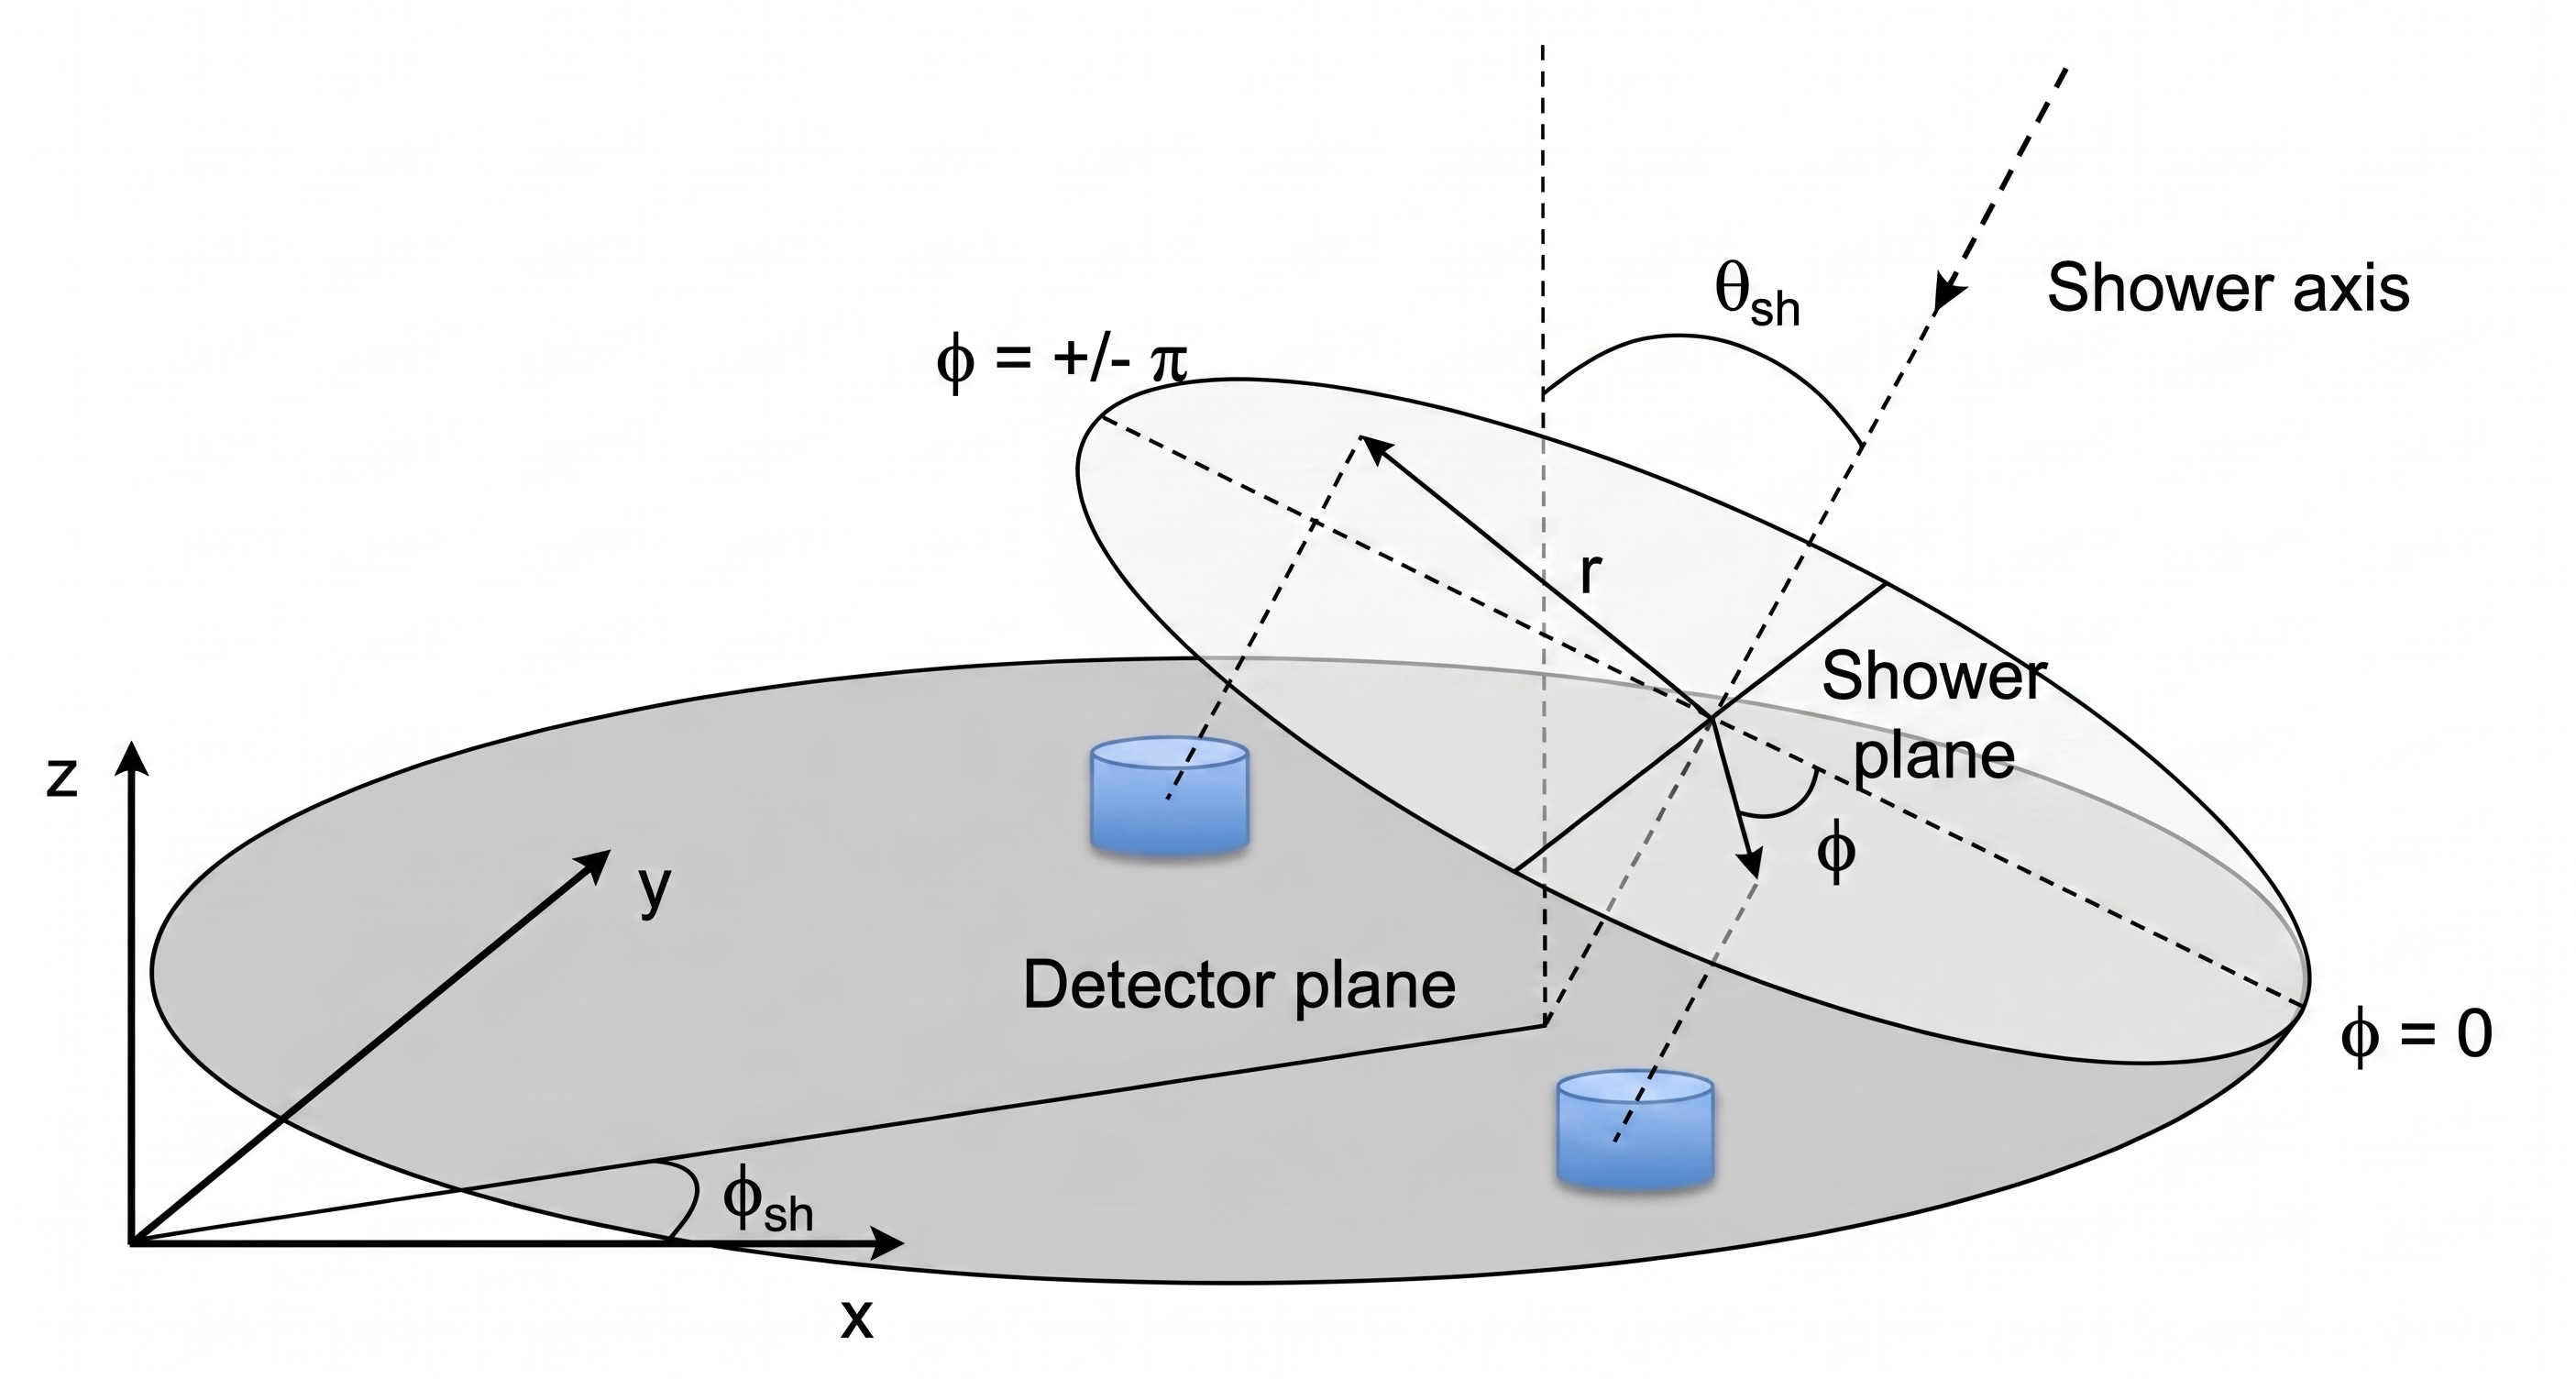
\includegraphics[width=1.08\textwidth]{esquema_lluvia.jpeg}}
  \end{columns}
  \note{%
    The asymmetry of the total SD signal in inclined showers is well known. The
    question here is what happens with muons alone, which is what the UMD gives us:
    shielded, so free of the electromagnetic component. The observable is the
    first-harmonic amplitude A1 of the muon density in the shower plane. For a vertical
    shower the density is circularly symmetric. When the shower is inclined, two regions
    appear: the early side, reached first through less atmosphere, and the late side,
    reached later through more atmosphere. A positive A1 means more muons on the early
    side. A1 is fitted on an ensemble of showers, not event by event.\par
    \textit{Transition:} We start in the cleanest setup we have.}
\end{frame}

\begin{frame}{Why an early--late asymmetry?}
  \small
  Four mechanisms modulate the muon density in the shower plane:
  \vspace{0.4em}
  \begin{center}
    \renewcommand{\arraystretch}{1.35}
    \begin{tabular}{p{3.3cm}p{7.6cm}l}
      \toprule
      \textbf{Mechanism} & \textbf{Effect} & \textbf{Favours}\\
      \midrule
      Atmospheric attenuation & The late region is farther: more muons decay on the way &
        \textcolor{plotBlue}{\textbf{early}}\\
      Detector response & Late muons arrive more inclined: a flat detector (UMD) sees a lower
        density there & \textcolor{plotBlue}{\textbf{early}}\\
      Kinematic divergence & At the same $r$, the late region is farther ($1/d^2$ dilution) but
        needs a smaller opening angle (smaller, more probable $p_t$) &
        \textcolor{plotBlue}{\textbf{early}} / \textcolor{plotMaroon}{\textbf{late}}\\
      Geomagnetic field & Separates $\mu^+$ and $\mu^-$; second order for $\theta\lesssim70^\circ$ &
        ---\\
      \bottomrule
    \end{tabular}
  \end{center}
  \vspace{0.3em}
  \centering A toy model combining them predicts \alert{$A_1>0$, growing with $r$ and $\theta$}.
  \note{%
    [20--30 s] Four mechanisms shape the muon density in the shower plane. Attenuation and
    the response of a flat detector favour the early side, the kinematic divergence pulls
    both ways, and the geomagnetic field is second order at these angles. A toy model
    combining them predicts a positive A1, growing with distance and zenith angle.\par
    \textit{Transition:} Now the simulations.}
\end{frame}

% ============================================================
\section{The reference: Monte Carlo geometry}
% ============================================================

\begin{frame}{Simulations and the Dense Ring}
  \begin{columns}[c]
    \column{0.66\textwidth}
      \begin{itemize}
        \item Official CORSIKA + \emph{Offline} production, with SD-750 and UMD:
      \end{itemize}
      \vspace{0.1em}
      {\footnotesize
      \renewcommand{\arraystretch}{1.15}
      \hspace{1.2em}\begin{tabular}{@{}ll@{}}
        \textbf{Hadronic models} & SIBYLL~2.3e (main), QGSJET-III.01\\
        \textbf{Primaries} & p (main), He, Fe\\
        \textbf{Energy} & $10^{17.5}$--$10^{18}$~eV\\
        \textbf{Zenith angle} & $\theta\le65^\circ$\\
      \end{tabular}}
      \vspace{0.4em}
      \begin{itemize}
        \item \textbf{Dense Ring}: 12 virtual stations at $r=450$~m from the
          \textbf{true} axis, every $30^\circ$ in the shower plane. Same $r$ for all:
          the radial fall-off of the density cannot produce a modulation in $\phi$.
      \end{itemize}
    \column{0.30\textwidth}
      \centering
      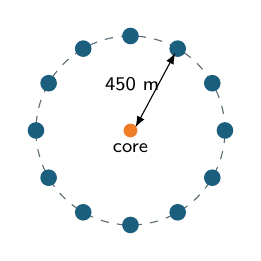
\begin{tikzpicture}[x=0.8cm,y=0.8cm]
        \draw[itedaGray, dashed] (0,0) circle (1.5);
        \foreach \angulo in {0,30,...,330}
          \fill[itedaTeal] (\angulo:1.5) circle (3pt);
        \fill[itedaOrange] (0,0) circle (2.5pt);
        \node[font=\scriptsize, below] at (0,-0.05) {core};
        \draw[{Latex[length=1.4mm]}-{Latex[length=1.4mm]}] (0.08,0.05) -- (60:1.42);
        \node[font=\scriptsize, anchor=east] at (50:0.95) {450 m};
      \end{tikzpicture}

      \vspace{0.3em}
      {\scriptsize Shower plane.}
  \end{columns}
  \note{%
    [20--30 s] Official collaboration production; most of what I show is protons with SIBYLL
    2.3e. We start with the Dense Ring: twelve virtual stations at 450 meters from the true
    axis, so the fall of the density with distance cannot fake a modulation.\par
    \textit{Transition:} This is what the muon density looks like on the ring.}
\end{frame}

\begin{frame}{A clear modulation on the Dense Ring}
  \badgeAD
  \begin{columns}[c]
    \column{0.60\textwidth}
      \hspace*{-0.5cm}%
      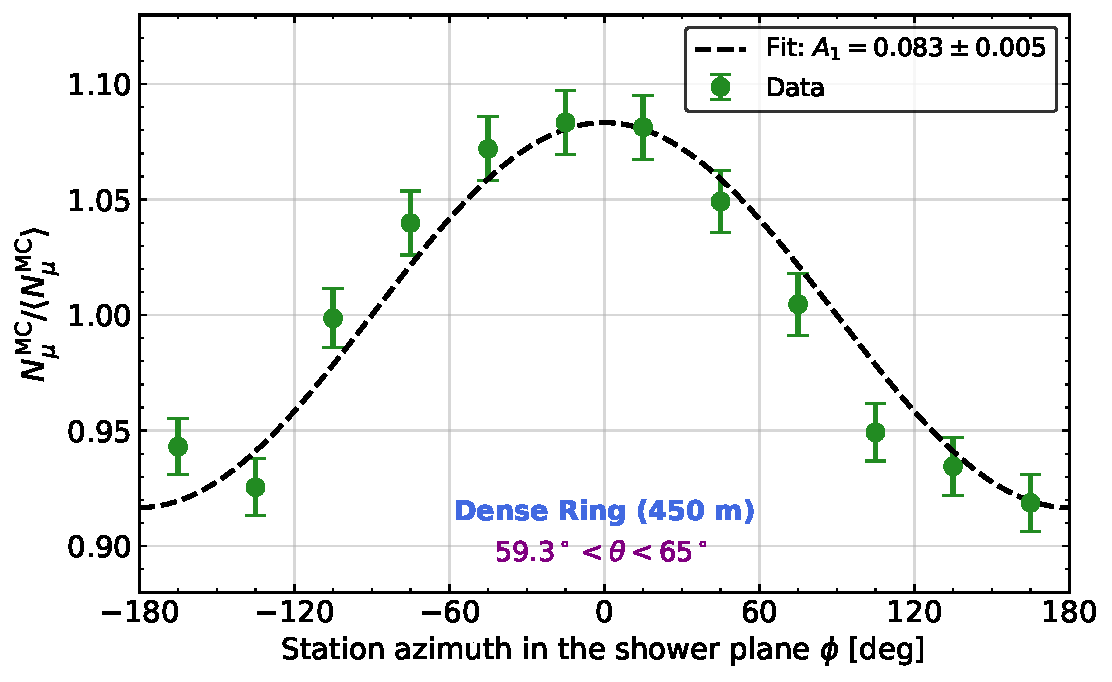
\includegraphics[width=1.04\textwidth,height=6.2cm,keepaspectratio]{DenseRing_Fit_UMD_MC_EN.pdf}
    \column{0.38\textwidth}
      \begin{itemize}
        \item Injected muon number $N_\mu^{\text{MC}}$, $59.3^\circ<\theta<65^\circ$.
        \item Maximum in the \early{} region ($\phi\approx0$).
        \item Early--late difference \alert{$\approx17\%$} peak to peak
          ($\pm8\%$ around the mean).
      \end{itemize}
  \end{columns}
  \note{%
    Here are the twelve ring stations for the most inclined bin, using the injected
    muon numbers. The density peaks on the early side and the first harmonic gives an
    amplitude of 0.083: the early side has about eight percent more muons than the
    mean, the late side eight percent fewer. With the reconstructed muon numbers the
    same bin gives 0.068; that difference is the counting reconstruction, in the
    backup. (If asked: the Dense Ring zenith bins are in reconstructed zenith angle.)\par
    \textit{Transition:} How does it change with zenith angle?}
\end{frame}

\begin{frame}{Comparison: SD vs.\ UMD on the Dense Ring}
  \badgeAD
  \begin{columns}[c]
    \column{0.64\textwidth}
      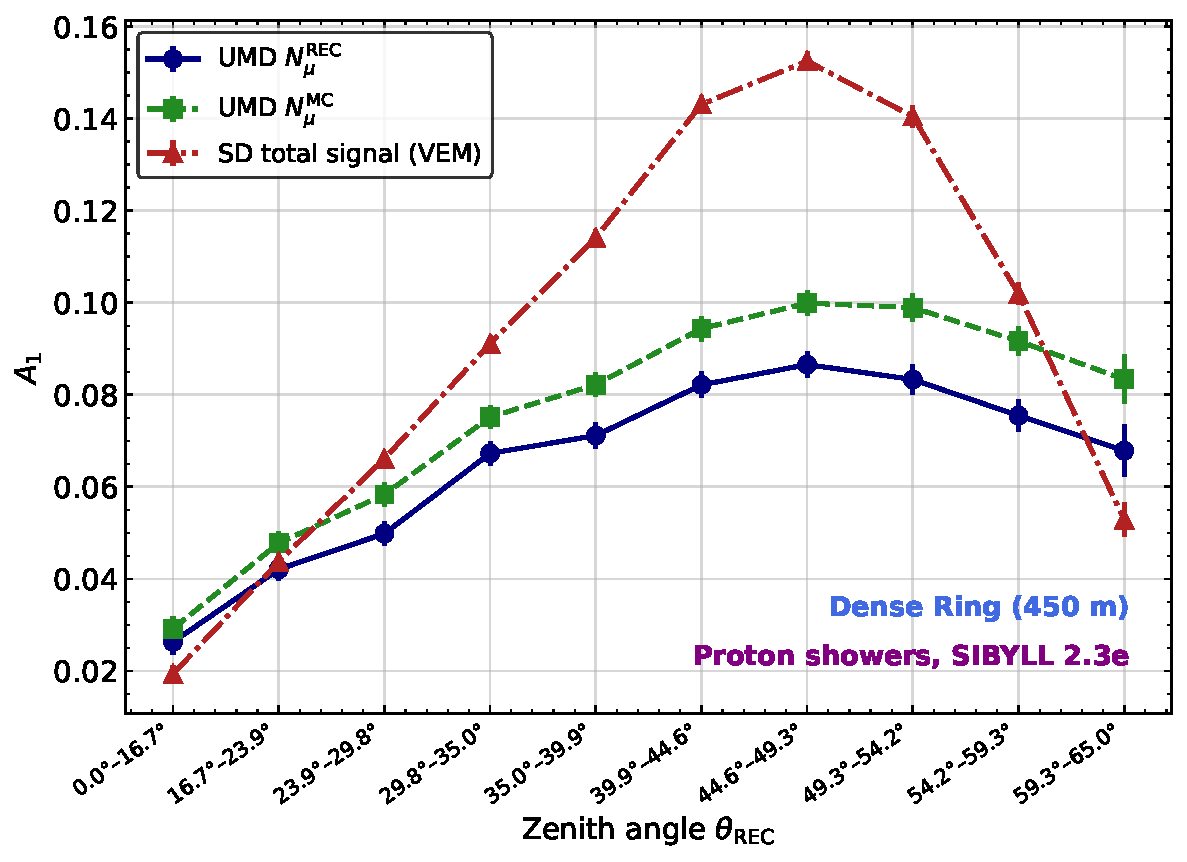
\includegraphics[width=\textwidth]{DenseRing_A1_vs_Theta_EN.pdf}
    \column{0.34\textwidth}
      \footnotesize
      \setbeamerfont{itemize/enumerate body}{size=\footnotesize}
      \begin{itemize}
        \setlength{\itemsep}{2pt}
        \item UMD: $A_1>0$, grows with $\theta$ up to $\sim45$--$50^\circ$.
        \item UMD: lower amplitude with reconstructed ($N_\mu^{\text{REC}}$) than with
          injected ($N_\mu^{\text{MC}}$) muons, same shape.
        \item SD total signal: larger than the UMD at $\sim20$--$60^\circ$
          (EM-dominated); drops sharply above $\sim50^\circ$.
        \item SD below the UMD only at $\theta\gtrsim60^\circ$.
      \end{itemize}
  \end{columns}
  \note{%
    [20--30 s] The muon asymmetry grows with zenith angle. The SD total signal is larger,
    because it is dominated by the electromagnetic part, and falls below the UMD only above
    about sixty degrees.\par
    \textit{Transition:} For the radial dependence we need the real Infill array.}
\end{frame}


\begin{frame}{UMD radial dependence on the Infill (MC geometry)}
  \badgeIF
  \vspace{-0.4em}
  {\small Real Infill stations (750~m): the distance to the axis varies from station to station
  $\Rightarrow$ $A_1(r)$. Station $r$ and $\phi$ depend on where the axis is: here the
  \textbf{true} core and direction.}
  \vspace{0.2em}
  \begin{columns}[c]
    \column{0.62\textwidth}
      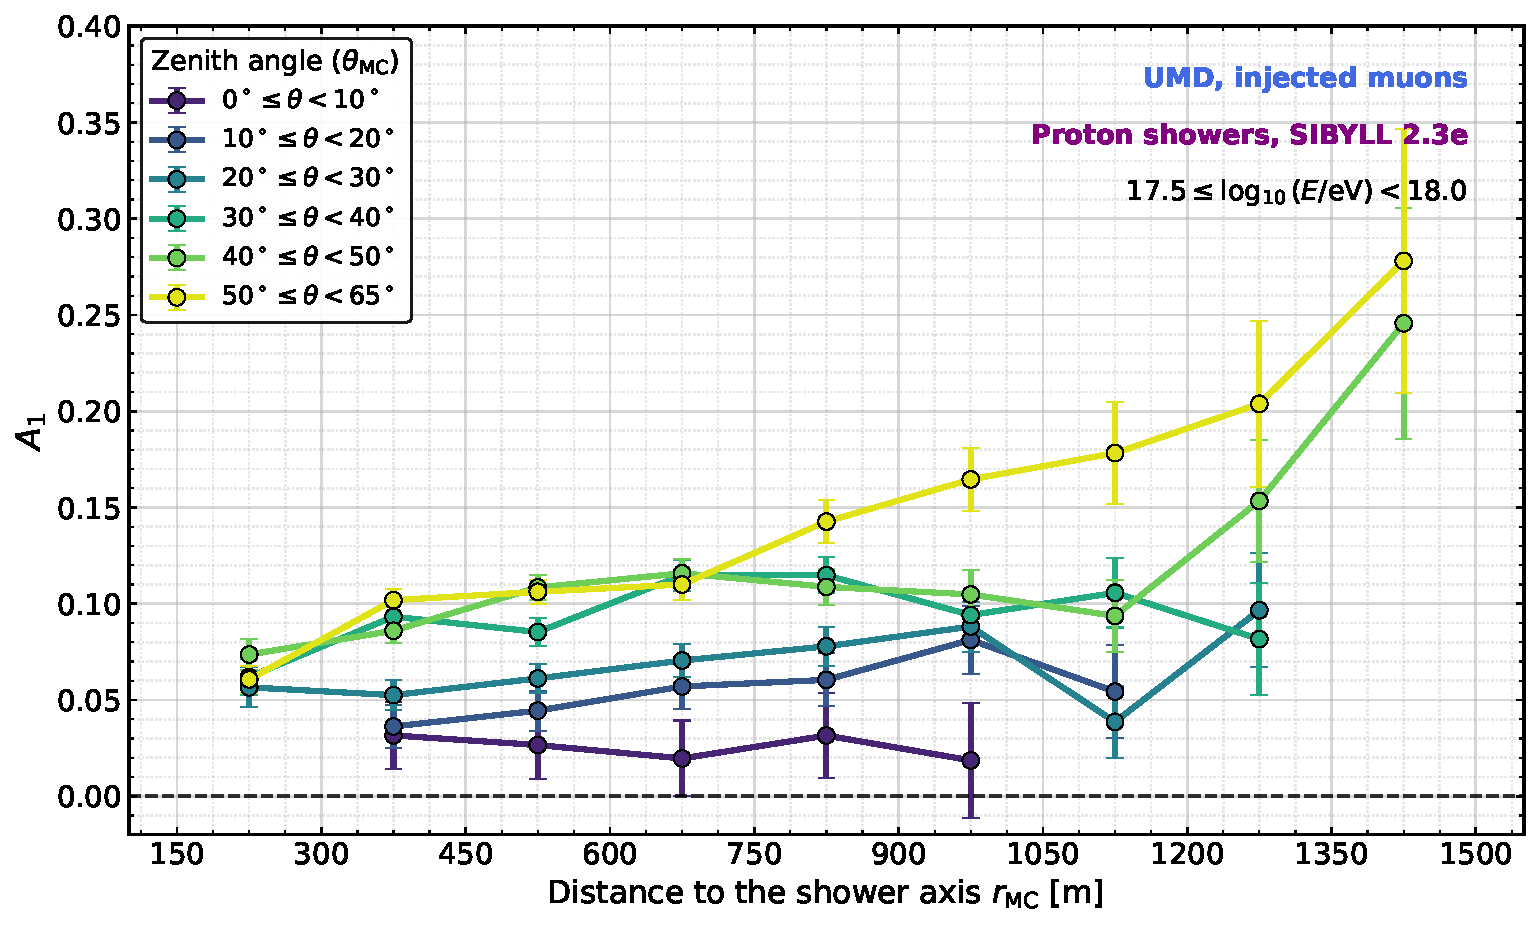
\includegraphics[width=\textwidth]{Infill_UMD_A1_vs_r_MC_EN.pdf}
    \column{0.36\textwidth}
      \footnotesize
      \setbeamerfont{itemize/enumerate body}{size=\footnotesize}
      \begin{itemize}
        \setlength{\itemsep}{2pt}
        \item \textbf{UMD only} (injected muons).
        \item Radial bins of $\Delta r=150$~m; zenith bins of $10^\circ$.
        \item $\theta<10^\circ$: compatible with zero.
        \item $10$--$40^\circ$: grows with $r$, then \textbf{flattens}.
        \item $\theta\ge40^\circ$: \textbf{grows with $r$}.
      \end{itemize}
      \vspace{0.3em}
      \centering\alert{\textbf{This is our reference.}}
  \end{columns}
  \note{%
    Still simulations, but now with the real Infill stations. Their distances to the axis
    vary, so we can follow A1 as a function of r. The distance and azimuth of each station
    depend on where the shower axis is: we can use the true core and direction from the
    simulation, or the reconstructed ones, and the main difference between the two is the
    core position. Here we use the true one. This is the UMD alone, with the injected muon
    numbers, in radial bins of 150 meters and zenith bins of ten degrees. Near-vertical
    showers show no significant asymmetry. Between ten and forty degrees it grows with
    distance and then flattens. Above forty degrees it grows with distance. (If asked:
    at forty to fifty degrees it stays around 0.1 and rises only beyond about twelve
    hundred meters, where the statistics are lower.) This is what an ideal analysis
    should find.\par
    \textit{Transition:} Now we compare with the surface detector in the same
    showers.}
\end{frame}

% ============================================================
\section{The SD inversion and the selection bias}
% ============================================================

\begin{frame}{The SD comparison: inversion far from the core}
  \badgeIF
  \begin{columns}[c]
    \column{0.66\textwidth}
      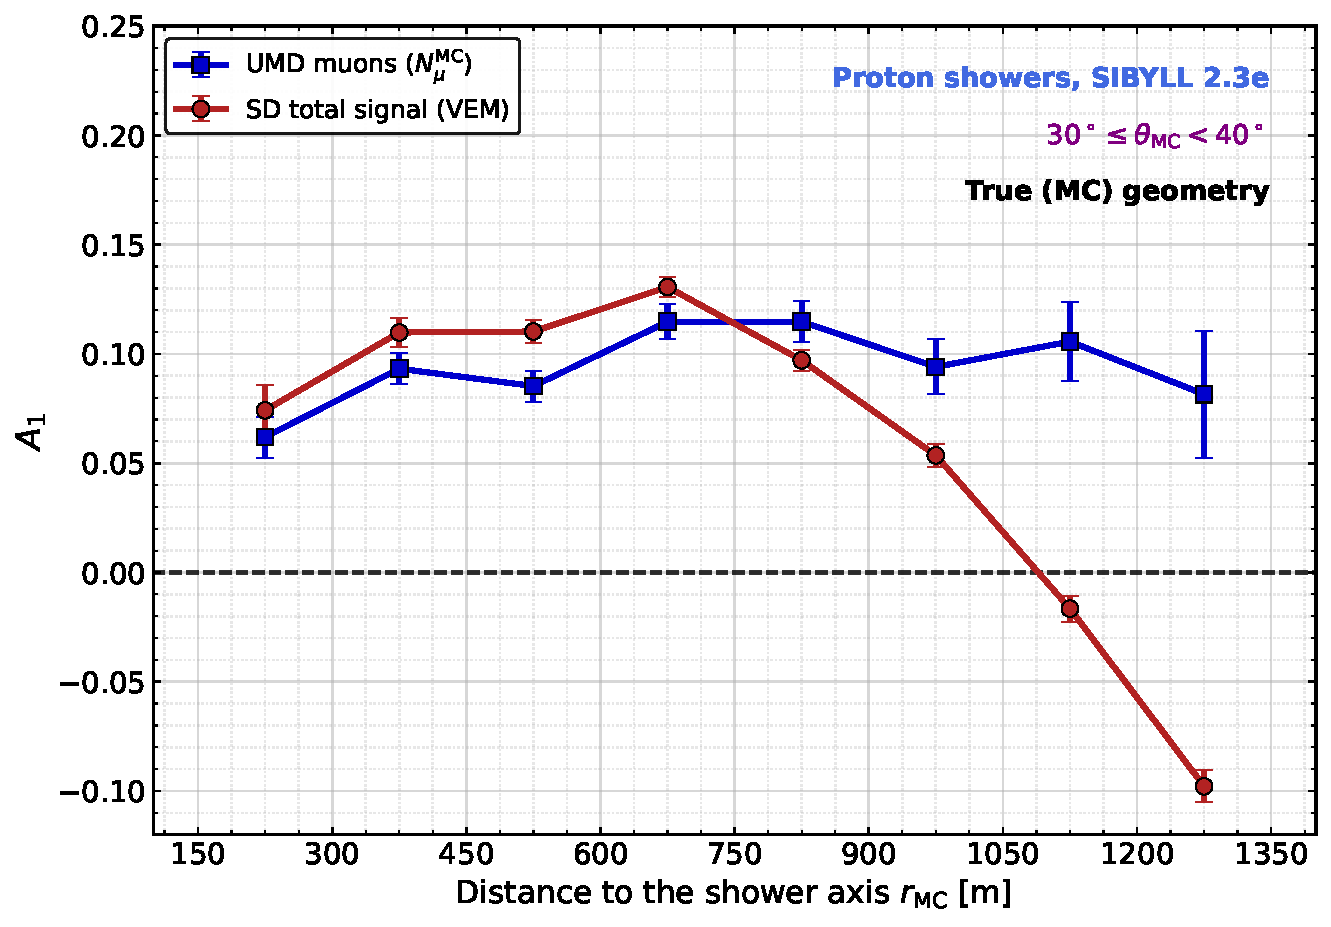
\includegraphics[width=\textwidth]{Infill_UMD_vs_SD_Total_EN.pdf}
    \column{0.32\textwidth}
      \begin{itemize}
        \item We now compare the UMD and SD asymmetries in the same Infill showers.
        \item MC geometry, $30^\circ\le\theta<40^\circ$.
        \item UMD: positive at all $r$.
        \item SD total: a maximum, then \alert{negative} far from the core.
      \end{itemize}
  \end{columns}
  \note{%
    Now we compare the UMD with the surface detector, on the same Infill showers and
    with the same true geometry. The UMD stays positive at all distances. The total SD
    signal peaks, then decreases, and far from the core becomes clearly negative, an
    excess on the late side. Since the core and direction are the true ones, this
    cannot be a reconstruction error.\par
    \textit{Transition:} Which part of the tank signal is responsible?}
\end{frame}

\begin{frame}[t]{It is the SD muon component that inverts}
  \badgeIF
  \vspace{-0.6em}
  \begin{columns}[T]
    \column{0.62\textwidth}
      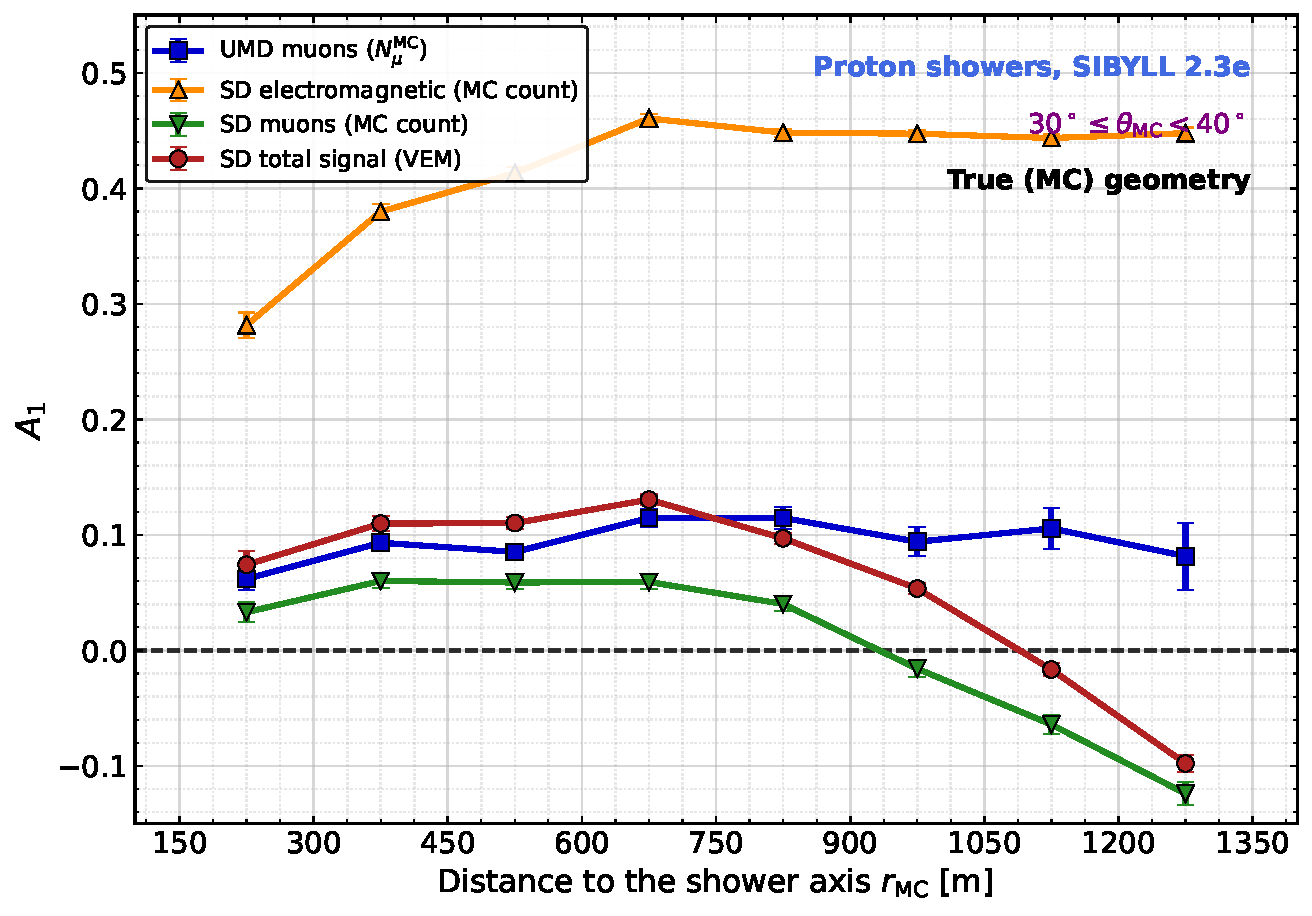
\includegraphics[width=\textwidth]{Infill_SD_Breakdown_vs_UMD_EN.pdf}
    \column{0.36\textwidth}
      \begin{itemize}
        \item MC particle counts in the tank, split by component.
        \item \textcolor{itedaOrange}{\textbf{EM}}: positive at all $r$.
        \item \textcolor{plotGreen}{\textbf{SD muons}}: positive near the core,
          \alert{negative} beyond $\sim900$~m.
        \item The SD total follows its muons at large $r$.
      \end{itemize}
      \vspace{0.3em}
      \centering\alert{\textbf{Same quantity, opposite sign in UMD and SD.}}
  \end{columns}
  \note{%
    Splitting the tank signal with the simulation truth, the electromagnetic part is
    positive everywhere. The muon part is what inverts, and the total SD signal
    follows it far from the core. So we compare the same physical quantity, muons
    crossing a detector, and get opposite signs in the UMD and in the SD. Our
    analytic model of muon propagation does not produce a negative asymmetry at these
    distances, so we looked at how the observable is built.\par
    \textit{Transition:} The key point: we never average over all stations.}
\end{frame}



\begin{frame}{Without \texttt{HasStation}, the inversion disappears}
  \badgeIF
  \vspace{-0.8em}
  \begin{columns}[c]
    \column{0.62\textwidth}
      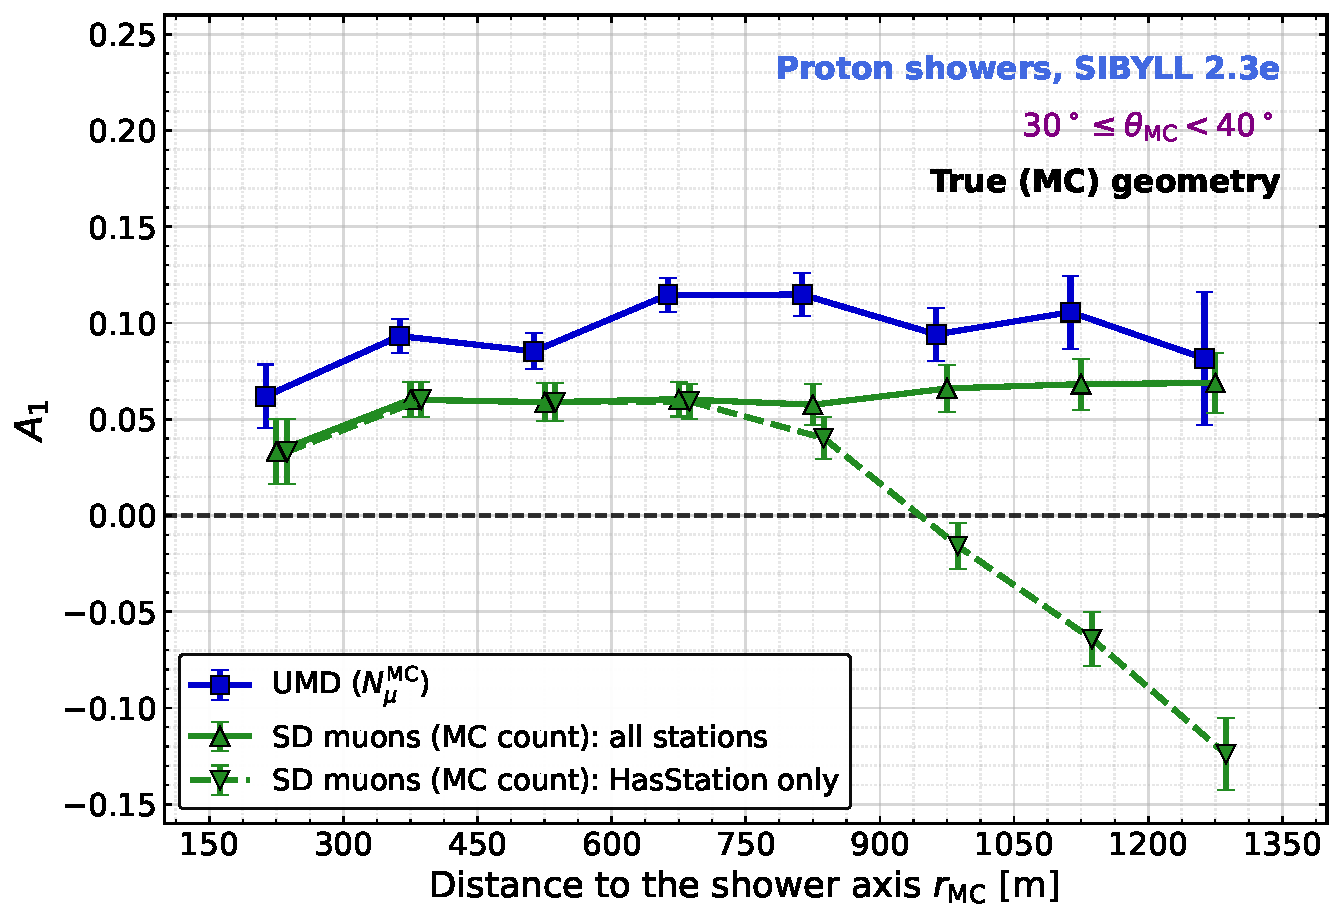
\includegraphics[width=\textwidth]{Selection_Test1_EN.pdf}
    \column{0.36\textwidth}
      \begin{itemize}
        \item Same MC counts, coordinates and fit: only \textbf{which stations}
          enter changes.
        \item All stations: SD muons \textbf{positive at all $r$}
          ($+0.03$ to $+0.07$).
        \item Same sign and trend as the UMD, \textbf{but not the same values}.
      \end{itemize}
  \end{columns}
  \note{%
    Every curve so far is an average over the stations that belong to the reconstructed
    event. If the chance of being kept depends on the station's own muon content, and
    differently on the early and late sides, the averages are biased. The direct test:
    same Monte Carlo muon counts in the tanks, same coordinates, same fit; only which
    stations enter changes. Over all simulated stations the SD muon asymmetry is
    positive at all distances, between plus three and plus seven percent. Requiring
    the station to be in the reconstructed event changes nothing up to about 750
    meters, where practically every station is kept, and then drives the asymmetry
    down to minus 0.12 at twelve to thirteen hundred meters: plus 0.069 plus or minus
    0.016 over all stations, against minus 0.124 plus or minus 0.019 with the
    requirement. The errors come from a bootstrap over the 960 showers, keeping the
    stations of each shower together. So the sign flip is a
    property of the station sample. Without the selection the SD muons have the same
    sign and trend as the UMD, but between 150 and 900 meters the UMD is still 0.03 to
    0.06 higher, and that difference excludes zero at 95 percent (backup slide);
    detector response and threshold are candidates, this is open.\par
    (If asked whether it is the trigger: the excluded tanks hold at most one muon in
    93 to 95 percent of the cases, backup.)\par
    \textit{Transition:} So far, true core and direction. In real data we only have the
    reconstructed ones.}
\end{frame}


% ============================================================
\section{Reconstructed geometry and the core position}
% ============================================================

\begin{frame}{REC geometry suppresses the asymmetry near the core}
  \badgeIF
  \begin{columns}[c]
    \column{0.62\textwidth}
      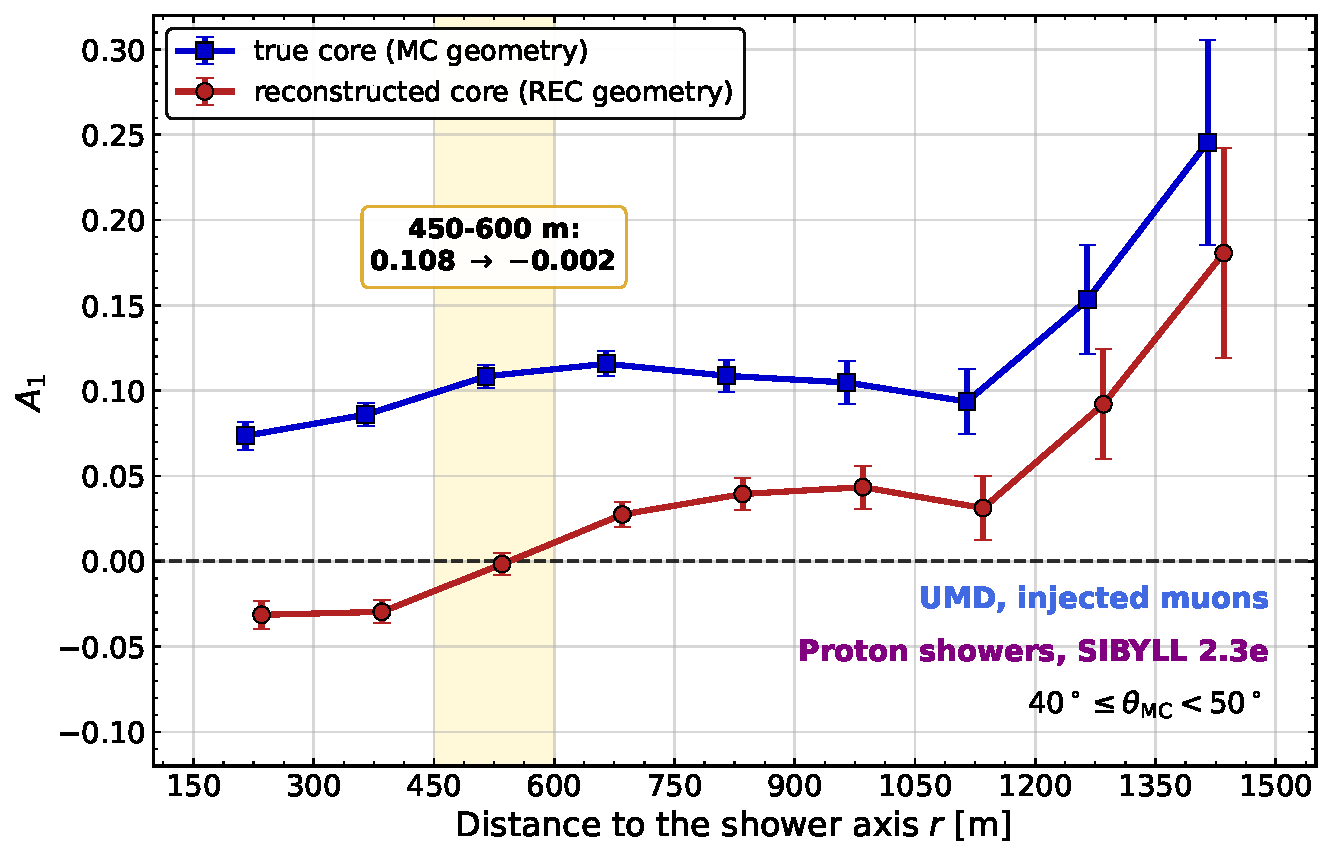
\includegraphics[width=\textwidth]{Rec_vs_MC_A1_vs_r_40_50_EN.pdf}
    \column{0.36\textwidth}
      \centering
      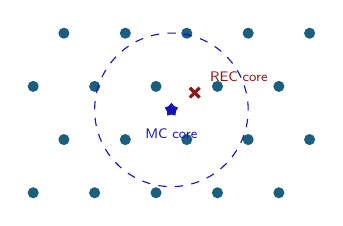
\begin{tikzpicture}[x=0.78cm,y=0.78cm]
        \foreach \fila in {0,1,2,3} {
          \foreach \col in {0,1,2,3,4} {
            \pgfmathsetmacro{\xpos}{\col + 0.5*mod(\fila,2)}
            \pgfmathsetmacro{\ypos}{0.866*\fila}
            \fill[itedaTeal] (\xpos,\ypos) circle (2.0pt);
          }
        }
        \node[star, star points=5, fill=plotBlue, inner sep=1.2pt] at (2.25,1.35) {};
        \node[font=\tiny, plotBlue, anchor=north] at (2.25,1.20) {MC core};
        \draw[plotMaroon, very thick] (2.55,1.55) -- ++(0.16,0.16) (2.55,1.71) -- ++(0.16,-0.16);
        \node[font=\tiny, plotMaroon, anchor=south west] at (2.72,1.65) {REC core};
        \draw[plotBlue, dashed] (2.25,1.35) circle (1.25);
      \end{tikzpicture}

      \raggedright
      \footnotesize
      \setbeamerfont{itemize/enumerate body}{size=\footnotesize}
      \begin{itemize}
        \setlength{\itemsep}{1pt}
        \item Same UMD modules and \textbf{injected} muons; \textbf{only the core changes}.
        \item Near the core $A_1$ drops to \textbf{zero or below}; farther out the curves
          \textbf{converge}.
        \item The effect comes from the \textbf{offset between the true and the reconstructed
          core positions}.
      \end{itemize}
  \end{columns}
  \note{%
    This is the reference curve of slide eight, forty to fifty degrees, with the
    same UMD modules and the same injected muon numbers, now computed a second time with
    the reconstructed core. Near the core the asymmetry drops to zero or becomes negative:
    at 450 to 600 meters it goes from 0.108 to minus 0.002. Farther out the two curves
    approach each other: the loss is not global, it shrinks with distance. We also swapped
    the two quantities one at a time: using the reconstructed or the true azimuth gives the
    same A1 within 0.002, so everything comes from the distance to the reconstructed core.
    (If asked, other zenith bands at 450 to 600 meters: 0.061 to 0.011 at twenty to thirty
    degrees, 0.085 to 0.002 at thirty to forty.)\par
    \textit{Transition:} So where is the reconstructed core?}
\end{frame}

\begin{frame}[t]{The reconstructed core is shifted toward the early region}
  \badgeIF
  \vspace{-1.2em}
  \centering
  \makebox[\textwidth][c]{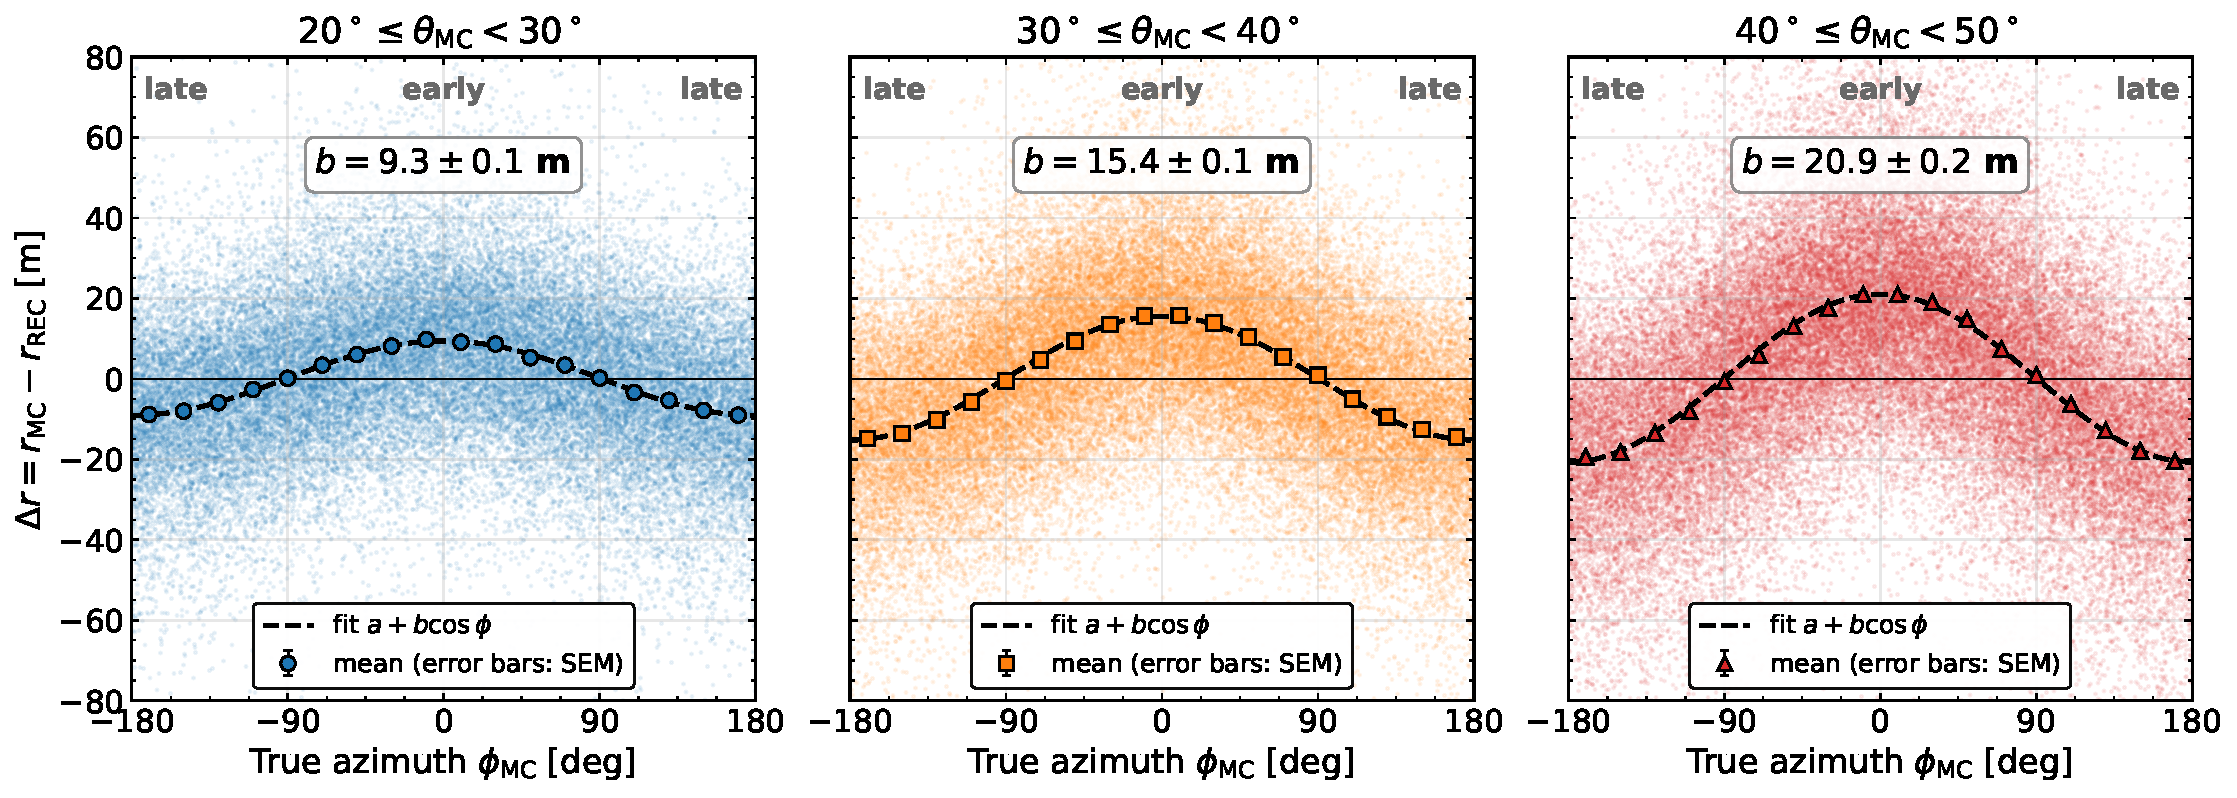
\includegraphics[width=1.06\textwidth,height=4.5cm,keepaspectratio]{Core_Shift_EN.pdf}}

  \vspace{0.1em}
  \raggedright
  \footnotesize
  \setbeamerfont{itemize/enumerate body}{size=\footnotesize}
  \begin{itemize}
    \setlength{\itemsep}{0pt}
    \item $\Delta r=r_{\text{MC}}-r_{\text{REC}}$ vs.\ $\phi$ is fitted by $a+b\cos\phi$, the
      modulation expected from a \textbf{rigid displacement of the core} by $b$: early stations
      are placed \textbf{closer} to the core, late ones \textbf{farther}; $a\simeq0.2$~m.
    \item Likely cause: the reconstruction LDF is \textbf{symmetric in $\phi$}; it absorbs
      the early excess by \textbf{moving the core toward the early side, where there is
      more signal}.
  \end{itemize}
  \note{%
    For each station we compare its distance to the true and to the reconstructed
    core, as a function of its true azimuth. If the core error were random, this
    would be flat. Instead it follows a cosine: early stations are placed closer to
    the core than they are, late stations farther. That is the signature of a
    systematic shift of the reconstructed core toward the early side: if the core is
    displaced rigidly by b toward the early direction, to first order every station's
    distance changes by b cos phi, which is exactly the fitted form. The constant a comes
    out at about 0.2 meters, so there is no azimuth-independent radial bias. The error bars
    are the standard error of the mean in each azimuth bin, smaller than the markers; the
    cloud behind them is the station-by-station spread, about twenty meters. So the
    modulation is very well determined even though single stations scatter a lot. The fitted shift is 9.3, 15.4 and 20.9 meters, with errors of
    0.1 to 0.2 meters. (If asked: those errors treat the stations as independent, but the
    stations of one shower share the same core error, so they are underestimated; a
    bootstrap over events is pending. The trend with zenith angle is far larger than
    any plausible error.) A likely reason: the LDF
    used in the reconstruction is symmetric in azimuth. Faced with more signal on the
    early side, the only thing the fit can do is move the core toward it. (Infill
    stations with reconstructed distance below 1400 meters.)\par
    \textit{Transition:} What does a shift of this size do to the LDF, and to A1?}
\end{frame}

\begin{frame}{A shifted core adds a $\cos\phi$ term to the LDF}
  \badgeIF
  \vspace{-0.4em}
  \begin{itemize}
    \item Binned by $r_{\text{REC}}$, a station at $r$ is really at $r+b\cos\phi$: its density
      belongs to \textbf{another radius}.
  \end{itemize}
  \vspace{-0.4em}
  \begin{equation*}
    \rho(r+b\cos\phi)\simeq\rho(r)\Big[1-\beta\,\frac{b}{r}\cos\phi\Big]
    \;\Rightarrow\;\boxed{\Delta A_1\simeq-\beta\,\frac{b}{r}}
    \qquad \beta=-\frac{\mathrm{d}\ln\rho}{\mathrm{d}\ln r}\ \text{(local)}
  \end{equation*}
  \centering
  {\footnotesize $450\le r<600$~m, injected muons}\\[0.2em]
  \renewcommand{\arraystretch}{1.1}
  \begin{tabular}{lcc|ccc}
    \toprule
    $\theta$ & $b$ [m] & $\beta$ & $\Delta A_1$ measured & $-\beta b/r$ predicted & residual\\
    \midrule
    $20$--$30^\circ$ & $9.3$  & $2.96$ & $-0.050$ & $-0.052$ & $+0.002$\\
    $30$--$40^\circ$ & $15.4$ & $2.72$ & $-0.084$ & $-0.080$ & $-0.004$\\
    $40$--$50^\circ$ & $20.9$ & $2.52$ & $-0.110$ & $-0.100$ & $-0.010$\\
    \bottomrule
  \end{tabular}

  \note{%
    [20--30 s] A shifted core puts each station at the wrong distance, and since the LDF is
    steep this adds a cos phi term of opposite sign: Delta A1 is about minus beta b over r.
    With b and beta measured on their own, the prediction matches the loss within 0.01.\par
    \textit{Transition:} Does this pattern show up in field data?}
\end{frame}


% ============================================================
\section{A first look at field data}
% ============================================================


\begin{frame}[t]{Field data follow the REC-geometry simulations}
  \badgeDATA
  \vspace{-1.0em}
  \centering
  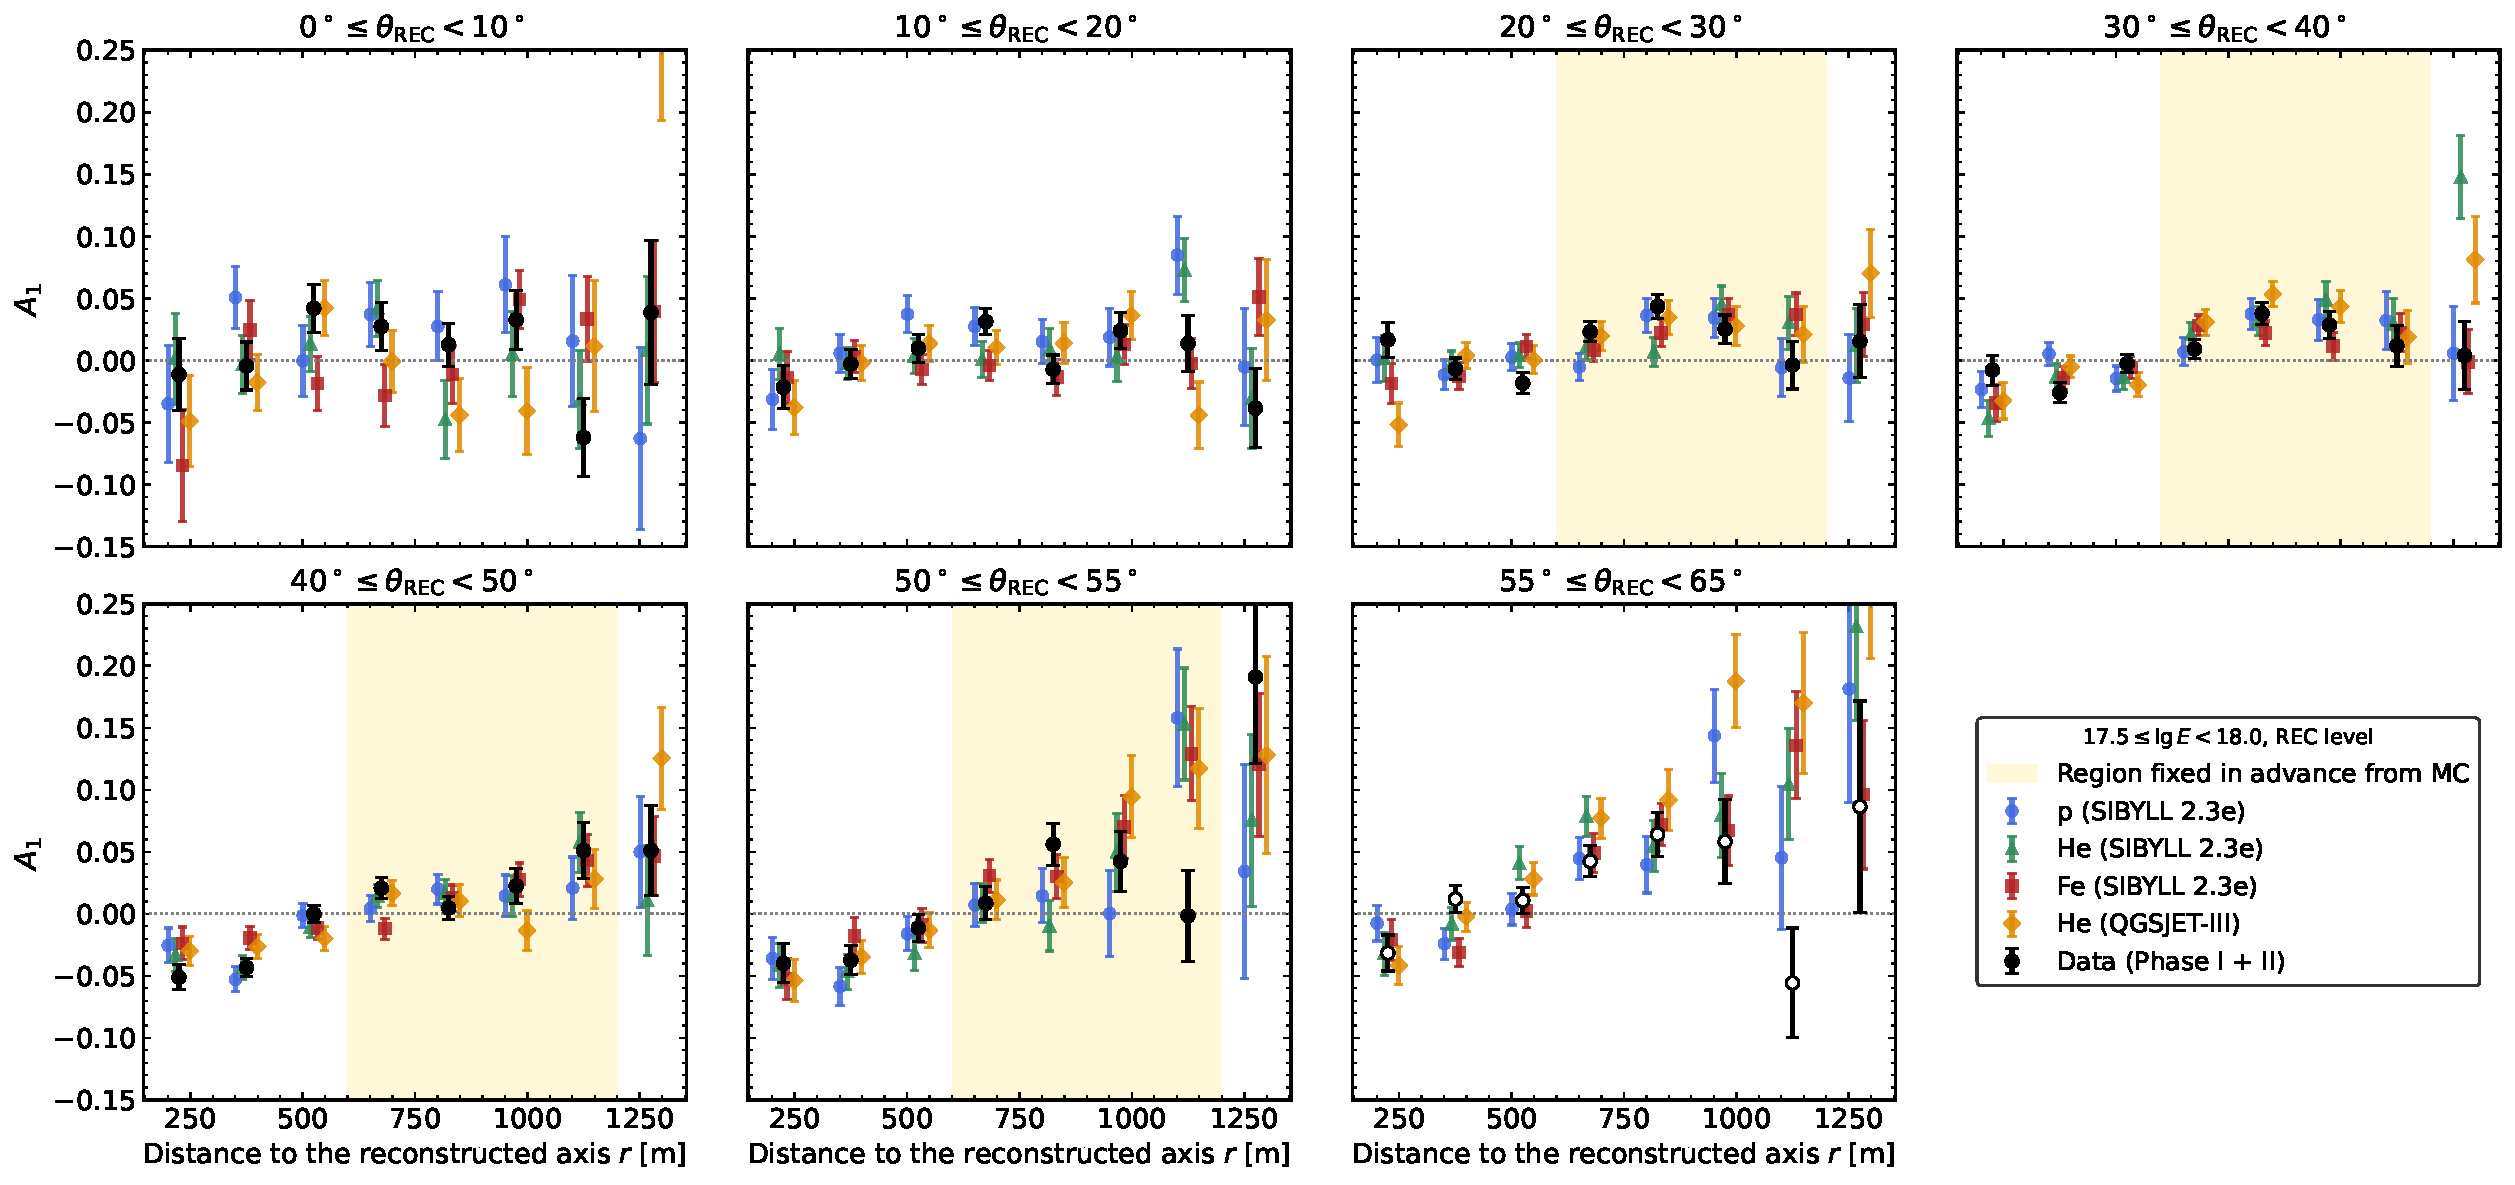
\includegraphics[width=0.97\textwidth,height=5.2cm,keepaspectratio]{FieldData_A1_vs_r_EN.pdf}

  \vspace{0.4em}
  \raggedright
  \footnotesize
  \setbeamerfont{itemize/enumerate body}{size=\footnotesize}
  \begin{itemize}
    \setlength{\itemsep}{0pt}
    \item Data (Phase I + II) and simulations with the \textbf{same reconstruction}, $17.5\le\lg E<18.0$.
    \item Same radial pattern: $A_1\le0$ near the core in inclined showers, positive farther out:
      the \textbf{signature of the core shift}, seen in data.
  \end{itemize}
  \note{%
    [20--30 s] Field data, in black, follow the simulations processed with the same
    reconstruction, including the negative asymmetry near the core in inclined showers:
    the core-shift signature, seen in data. (If asked for a single number: in the best
    Phase II cell A1 = 0.063 plus or minus 0.022, 2.8 sigma, backup.)\par
    \textit{Transition:} Let me summarize.}
\end{frame}

% ============================================================
\section{Conclusions}
% ============================================================

\begin{frame}{Conclusions}
  \begin{enumerate}
    \setlength{\itemsep}{0.6em}
    \item The UMD sees a \textbf{positive early--late muon asymmetry}.
    \item The SD inversion far from the core is \textbf{compatible with a station-selection
      effect}.
    \item The reconstructed core is \textbf{shifted toward the early region}, which suppresses
      $A_1$ near the core.
    \item The loss \textbf{is predicted by} $\Delta A_1\simeq-\beta\,b/r$.
    \item Field data \textbf{follow the REC-geometry simulations} (preliminary).
  \end{enumerate}
  \note{%
    Five points. The muon asymmetry is there. What we measure depends on how we build the
    observable: the SD inversion is compatible with a selection of the stations we average
    over, and the reconstructed core can erase the asymmetry near the core. The second effect is predicted by beta b over r,
    and the field data already show its signature. Next: parametrize b and beta with zenith
    angle and validate them on independent simulations, correct the field data, and separate
    trigger, readout and reconstruction inside HasStation.}
\end{frame}


\begin{frame}[plain]
  \begin{tikzpicture}[remember picture, overlay]
    \node[anchor=center, inner sep=0pt] at (current page.center)
      {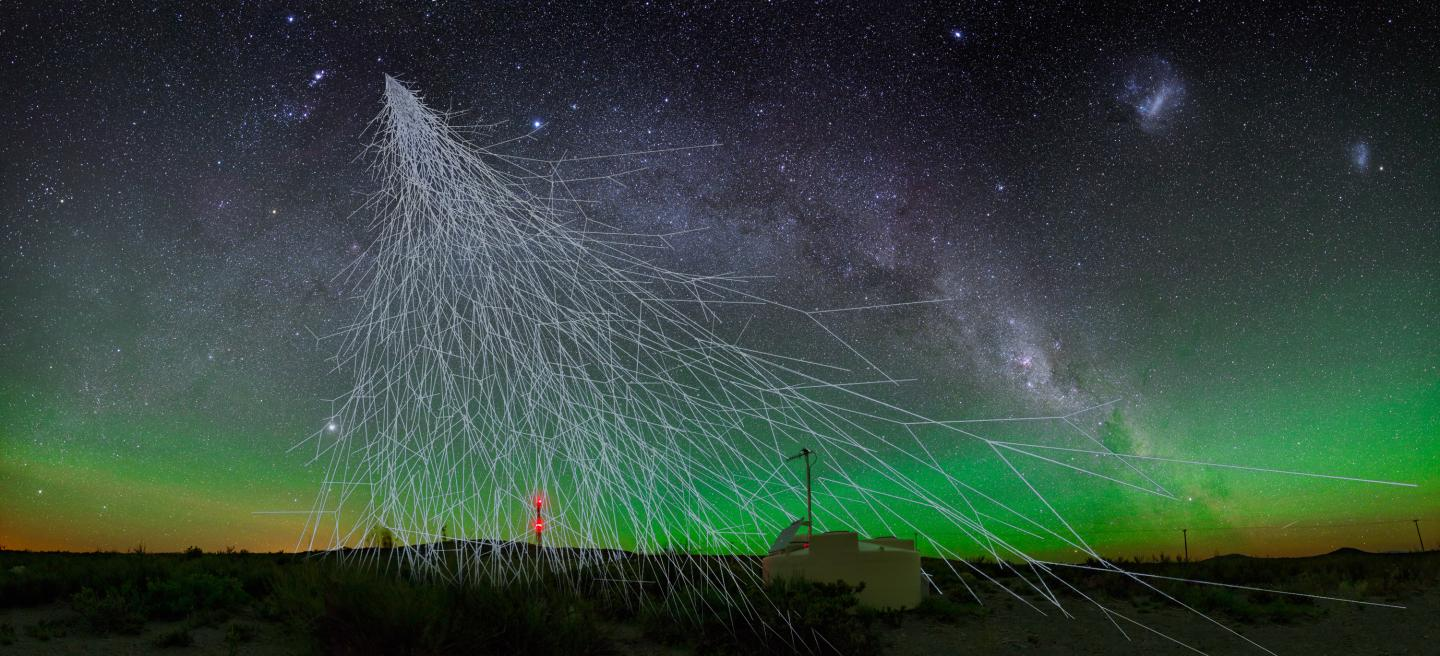
\includegraphics[height=\paperheight]{auger_cr.jpg}};
    \node[anchor=north east, xshift=-0.86cm, yshift=-0.49cm, text=black, opacity=0.6,
      font=\fontsize{34}{38}\selectfont\bfseries] at (current page.north east) {Thank you!};
    \node[anchor=north east, xshift=-0.9cm, yshift=-0.45cm, text=white,
      font=\fontsize{34}{38}\selectfont\bfseries] at (current page.north east) {Thank you!};
    \node[anchor=north east, xshift=-0.91cm, yshift=-1.79cm, text=black, opacity=0.6,
      font=\LARGE\bfseries] at (current page.north east) {Questions?};
    \node[anchor=north east, xshift=-0.95cm, yshift=-1.75cm, text=itedaOrange,
      font=\LARGE\bfseries] at (current page.north east) {Questions?};
    \node[anchor=south east, xshift=-0.15cm, yshift=0.1cm, text=white, opacity=0.8,
      font=\tiny] at (current page.south east)
      {Image: A.~Chantelauze, S.~Staffi, L.~Bret (Pierre Auger Observatory)};
  \end{tikzpicture}
\end{frame}

% ============================================================
\appendix
% ============================================================

\begin{frame}{Backup: the station selection biases the average}
  \badgeHYP
  \small
  A station enters the analysis only if it \textbf{belongs to the reconstructed
  event} (\texttt{HasStation}). If the probability that a station is kept depends on
  its own muon content, and this dependence is not the same on the early and late
  sides, the \textbf{regional averages are biased}.
  \vspace{0.3em}
  \begin{center}
  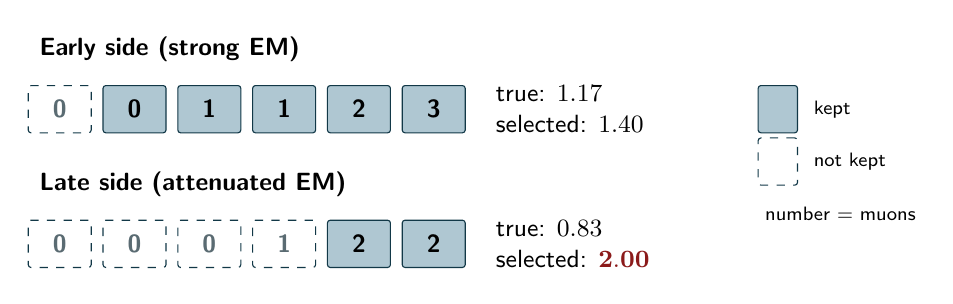
\begin{tikzpicture}[x=0.95cm,y=0.95cm,
      tank/.style={draw=itedaTealDark, minimum width=0.8cm, minimum height=0.6cm, rounded corners=1pt, font=\small\bfseries},
      on/.style={tank, fill=itedaTeal!35},
      off/.style={tank, fill=white, dashed, text=itedaGray}]
    \node[font=\small\bfseries, anchor=west] at (-0.4,1.2) {Early side (strong EM)};
    \node[off] at (0,0.4) {0};
    \foreach \x/\n in {1/0,2/1,3/1,4/2,5/3} {\node[on] at (\x,0.4) {\n};}
    \node[font=\small, anchor=west, align=left] at (5.7,0.4) {true: $1.17$\\ selected: $1.40$};
    \node[font=\small\bfseries, anchor=west] at (-0.4,-0.6) {Late side (attenuated EM)};
    \foreach \x/\n in {0/0,1/0,2/0,3/1} {\node[off] at (\x,-1.4) {\n};}
    \foreach \x/\n in {4/2,5/2} {\node[on] at (\x,-1.4) {\n};}
    \node[font=\small, anchor=west, align=left] at (5.7,-1.4) {true: $0.83$\\ selected: \textcolor{plotMaroon}{$\mathbf{2.00}$}};
    \node[on, minimum width=0.5cm] at (9.6,0.4) {};
    \node[font=\scriptsize, anchor=west] at (9.95,0.4) {kept};
    \node[off, minimum width=0.5cm] at (9.6,-0.3) {};
    \node[font=\scriptsize, anchor=west] at (9.95,-0.3) {not kept};
    \node[font=\scriptsize, anchor=west] at (9.3,-1.0) {number = muons};
  \end{tikzpicture}
  \end{center}
  \vspace{-0.2em}
  \centering Both averages go up, the late one much more: the sign flips
  \textbf{without moving a single muon}.
  \fuente{Illustrative cartoon. In the simulation, at 900--1500~m, 54\% of the early and 33\% of the late tanks are kept.}
  \note{%
    Every curve so far is an average over stations that are part of the reconstructed
    event. For the UMD that seemed natural, since it has no trigger of its own. But suppose
    the chance that a station is kept depends on how many muons it has. On the early side
    the electromagnetic signal is strong, so almost every station is kept, even one with no
    muons; only a few muon-poor ones are lost and the average goes up a little. On the late
    side the electromagnetic signal is weaker, so mostly the stations with more muons
    survive and the average goes up a lot. In this example the true averages are 1.17 and
    0.83, an early excess; the selected ones are 1.40 and 2.00, a late excess. The sign
    flips although no muon was created or moved. This is a hypothesis; the next two slides
    test it with the simulation.\par
    \textit{Transition:} The direct test is to remove the requirement.}
\end{frame}

\begin{frame}[t]{Backup: the excluded tanks hold very few muons}
  \badgeIF
  \vspace{-1.5em}
  \footnotesize
  \setbeamerfont{itemize/enumerate body}{size=\footnotesize}
  \begin{itemize}
    \item If the inversion comes from the \textbf{trigger}, the tanks dropped by the
      reconstruction (\texttt{HasStation} = False) should hold, on average,
      \alert{at most one muon}: too few for the station to trigger.
  \end{itemize}
  \vspace{-0.5em}
  \centering
  \makebox[\textwidth][c]{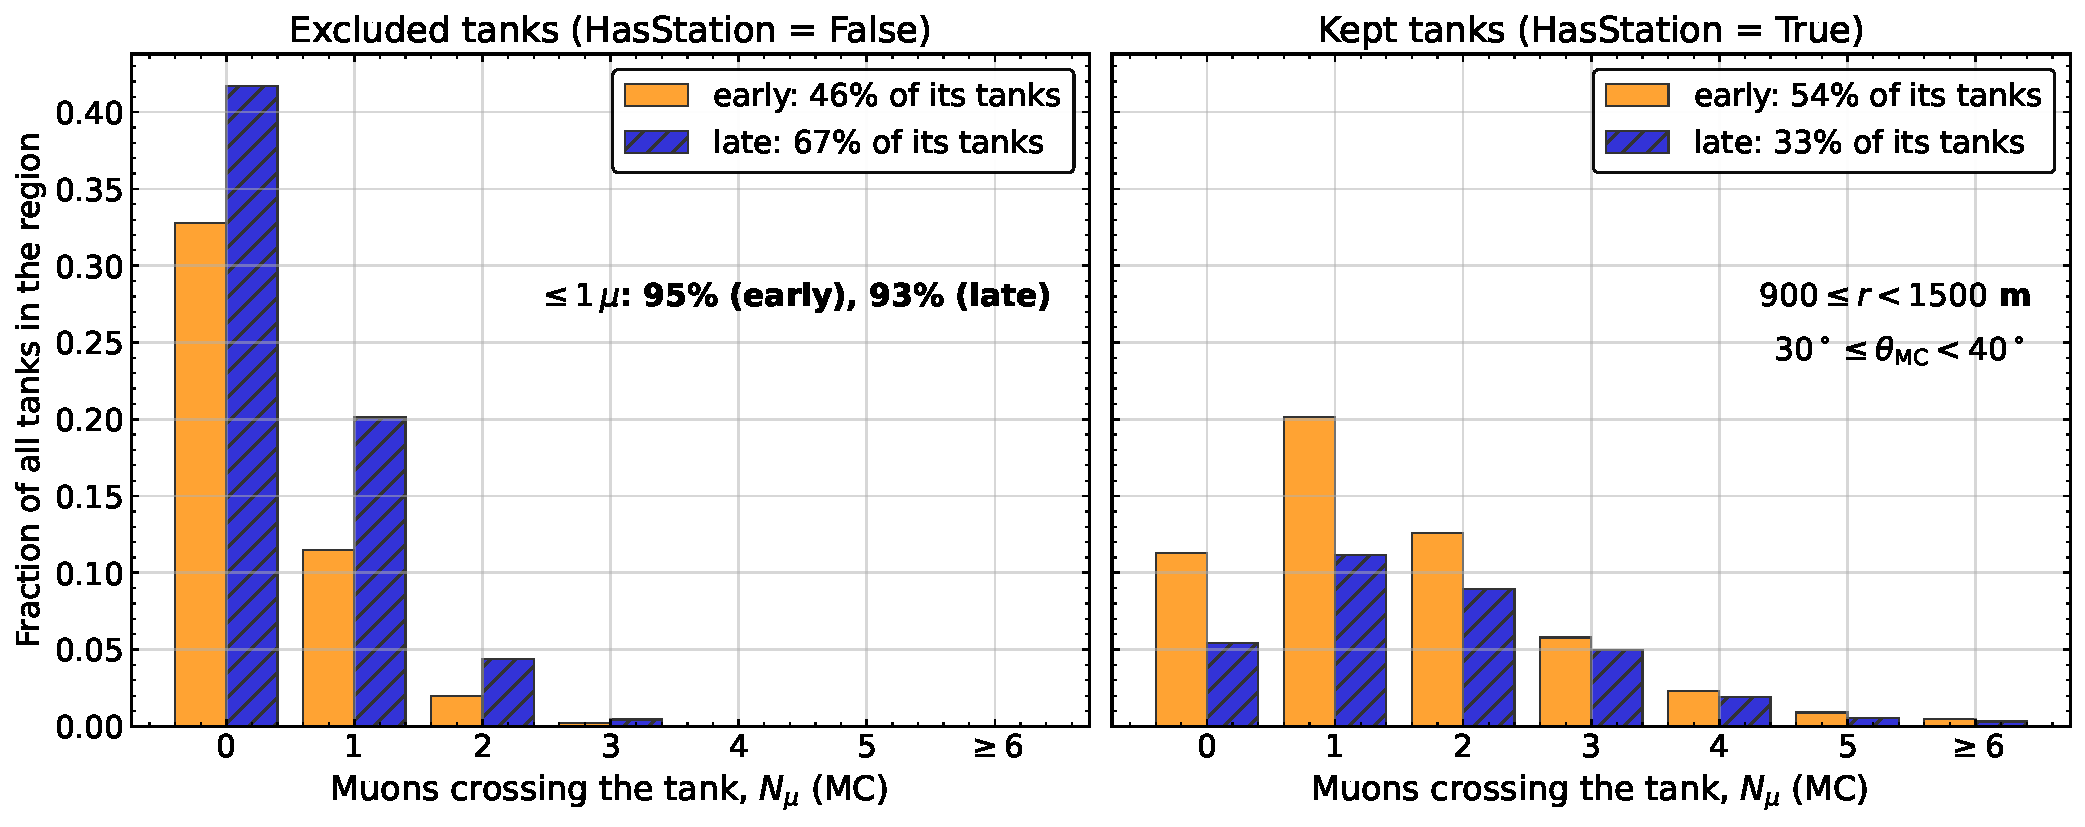
\includegraphics[width=1.02\textwidth,height=3.85cm,keepaspectratio]{Selection_Test2_EN.pdf}}

  {\scriptsize
  \renewcommand{\arraystretch}{1.0}
  \begin{tabular}{lccc}
    \toprule
    & $\langle N_\mu\rangle$ all tanks & $\langle N_\mu\rangle$ kept tanks & fraction kept\\
    \midrule
    \textcolor{plotBlue}{\textbf{early}} & $0.96$ & $1.49$ & $0.54$\\
    \textcolor{plotMaroon}{\textbf{late}} & $0.87$ & $1.69$ & $0.33$\\
    \bottomrule
  \end{tabular}}
  \note{%
    If the inversion is a trigger effect, there is a clear prediction: the tanks that
    the reconstruction drops should have been crossed by at most about one muon. If we
    found excluded tanks with several muons, a trigger explanation would not be
    credible. So we count the Monte Carlo muons in the tanks between 900 and 1500
    meters. Each region is normalised to all of its tanks, so the area of the bars is the
    fraction lost or kept: on the early side 46 percent of the tanks are dropped, on the
    late side 67 percent. Ninety-five percent of the excluded early tanks and ninety-three
    percent of the late ones have at most one muon. The table is the bias in numbers: over
    all tanks the early side has more muons, 0.96 against 0.87, which is the true positive
    asymmetry; over the kept tanks it is the other way round, 1.49 against 1.69. (If asked
    why the kept late tanks have more muons than the kept early ones: the selection
    raises both means, but much more on the late side, by a factor 1.9 against 1.55,
    because there the electromagnetic signal is weaker, about half, 14 against 28
    particles in the excluded tanks, so only muon-rich tanks pass; on the early side tanks
    with zero or one muon are often kept thanks to their electromagnetic signal. At 1200
    to 1350 meters only 18 percent of the late stations are kept, against 42 percent of
    the early ones.) This supports the trigger picture, but HasStation also includes
    readout and reconstruction, and we have not separated them, so it is consistent
    with a trigger effect, not a proof. (Early: $|\phi|<60^\circ$, late: $|\phi|>120^\circ$;
    MC geometry.)\par
    \textit{Transition:} So far, true core and direction. In real data we only have the
    reconstructed ones.}
\end{frame}

\begin{frame}{Backup: the modulation in one field-data cell}
  \badgeDATA
  \vspace{-0.8em}
  \begin{columns}[c]
    \column{0.62\textwidth}
      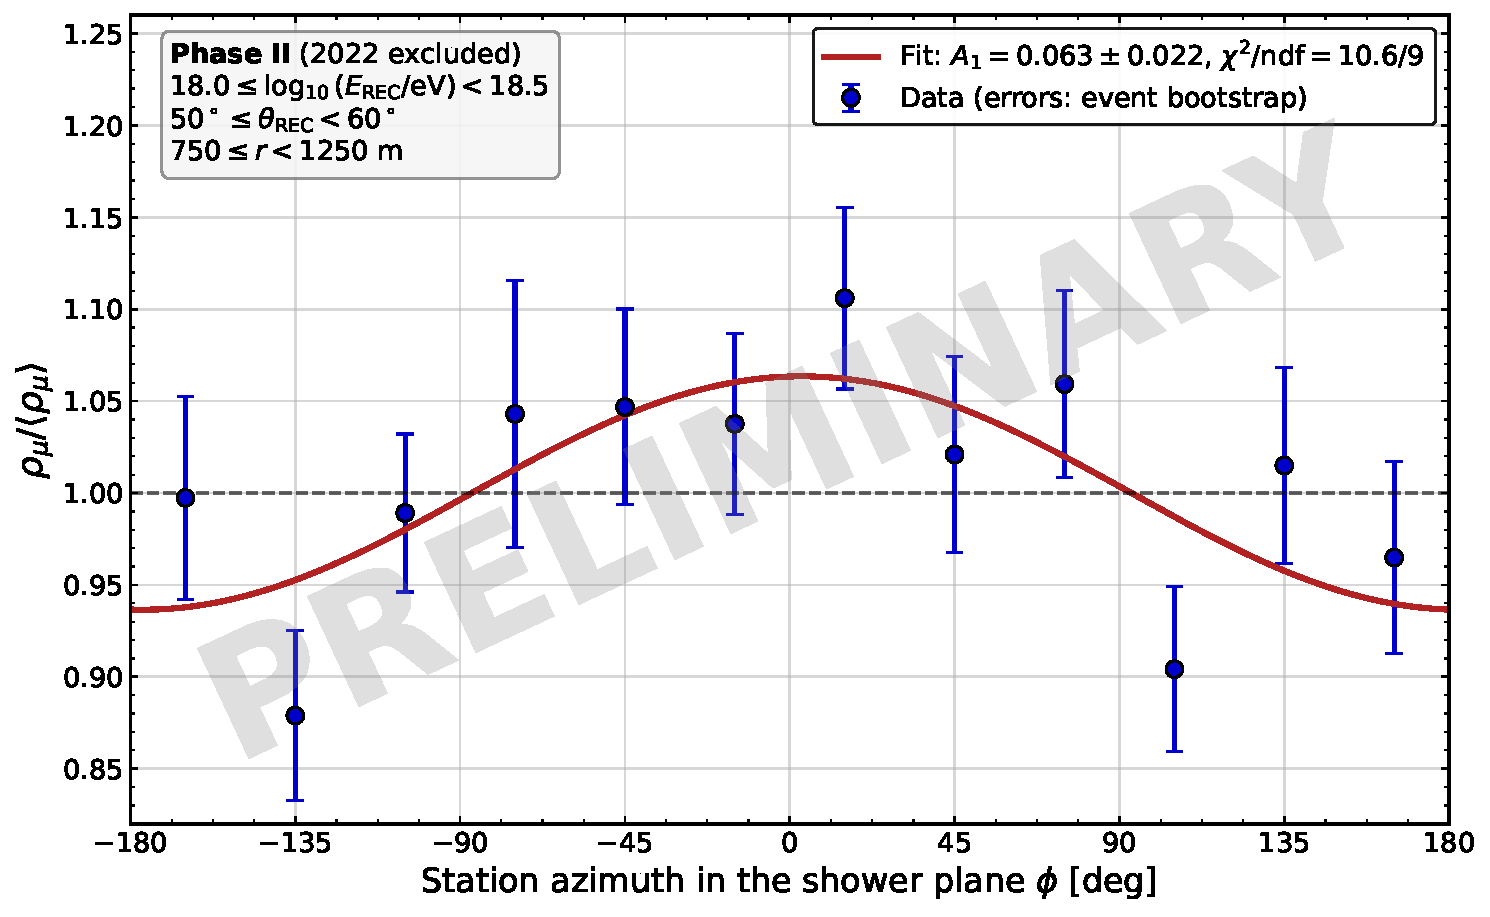
\includegraphics[width=\textwidth]{FieldData_PhaseII_Profile_EN.pdf}
    \column{0.36\textwidth}
      \footnotesize
      \setbeamerfont{itemize/enumerate body}{size=\footnotesize}
      \begin{itemize}
        \setlength{\itemsep}{2pt}
        \item UMD muon density vs.\ $\phi$, normalised to its mean, Phase~II; REC geometry.
        \item Maximum at $\phi\approx0$: \textbf{early excess}, as in the simulations.
        \item $A_1=0.063\pm0.022$ ($2.8\sigma$), $\chi^2/\mathrm{ndf}=10.6/9$; errors from a
          bootstrap over \textbf{events}.
        \item \textbf{Preliminary}: no core-shift correction, no systematics, no MC above
          $10^{18}$~eV.
      \end{itemize}
  \end{columns}
  \note{%
    This is the UMD muon density measured in the field, as a function of azimuth in the
    shower plane, for Phase II events in the cell shown in the box. The maximum is on the
    early side, as in the simulations. The first harmonic gives 0.063 plus or minus 0.022.
    That error comes from a bootstrap over events, because the modules of one shower are
    correlated; treating every module as independent gives 0.017, which overstates the
    significance. So this is a 2.8 sigma early excess, with a good fit. It is preliminary:
    the core correction we just discussed is not applied, there is no systematics study,
    and our simulations stop at ten to the eighteen. (If asked: part of the zenith range,
    55 to 60 degrees, is outside the standard SD-750 energy calibration; and 2022 Phase II
    commissioning data are excluded.)\par
    \textit{Transition:} And the radial pattern?}
\end{frame}

\begin{frame}{Backup: muon-counting reconstruction (MC geometry)}
  \badgeIF
  \begin{columns}[c]
    \column{0.60\textwidth}
      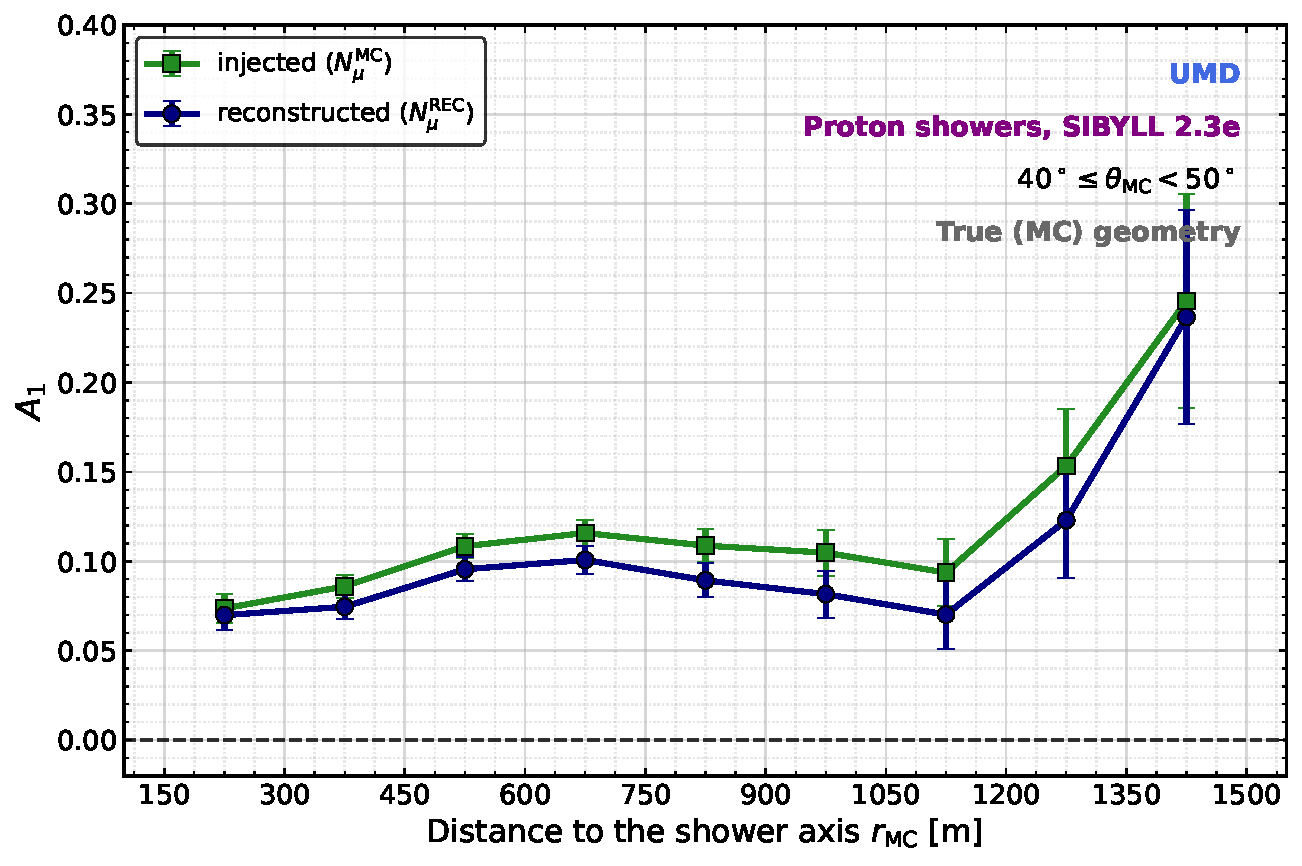
\includegraphics[width=\textwidth]{Backup_Counting_Infill_EN.pdf}
    \column{0.37\textwidth}
      \begin{itemize}
        \item $40^\circ$--$50^\circ$, true core and direction.
        \item The reconstructed muon number lowers $A_1$ by 5--23\%, with the same shape.
        \item A separate effect from the core shift.
      \end{itemize}
  \end{columns}
\end{frame}

\begin{frame}[t]{Backup: the counting bias depends on azimuth}
  \badgeAD
  \vspace{-0.8em}
  \centering
  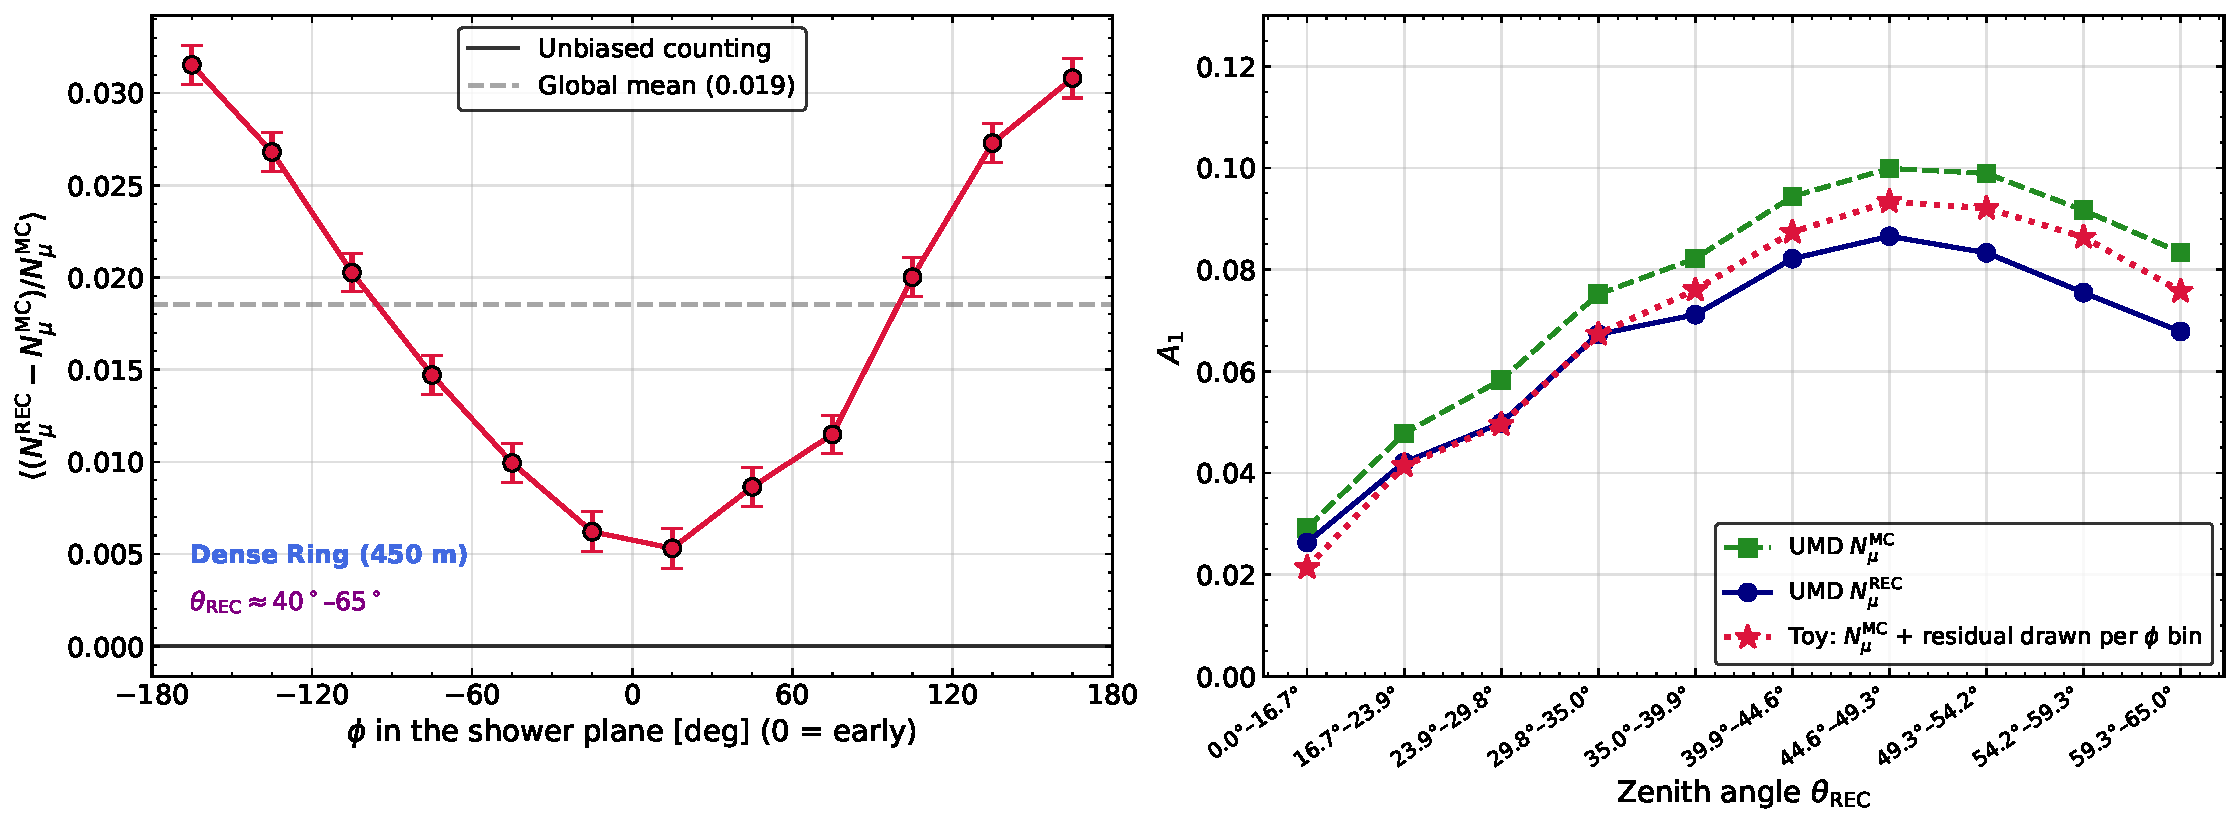
\includegraphics[width=\textwidth,height=4.6cm,keepaspectratio]{Backup_Counting_Bias_DenseRing_EN.pdf}

  \raggedright
  \footnotesize
  \setbeamerfont{itemize/enumerate body}{size=\footnotesize}
  \begin{itemize}
    \setlength{\itemsep}{0pt}
    \item Left: mean relative residual $(N^{\text{REC}}-N^{\text{MC}})/N^{\text{MC}}$ vs.\ $\phi$:
      $\approx0.005$ early, $\approx0.03$ late. More over-counting where there are fewer muons
      $\Rightarrow$ lower $A_1$.
    \item Right: injecting the residuals drawn per $\phi$ bin into $N_\mu^{\text{MC}}$ reproduces
      $A_1^{\text{REC}}$ up to $\theta\approx35^\circ$; above, half to two thirds of the loss.
      The remnant is open.
  \end{itemize}
\end{frame}


\begin{frame}{Backup: fit quality on the Dense Ring}
  \badgeAD
  \begin{columns}[c]
    \column{0.60\textwidth}
      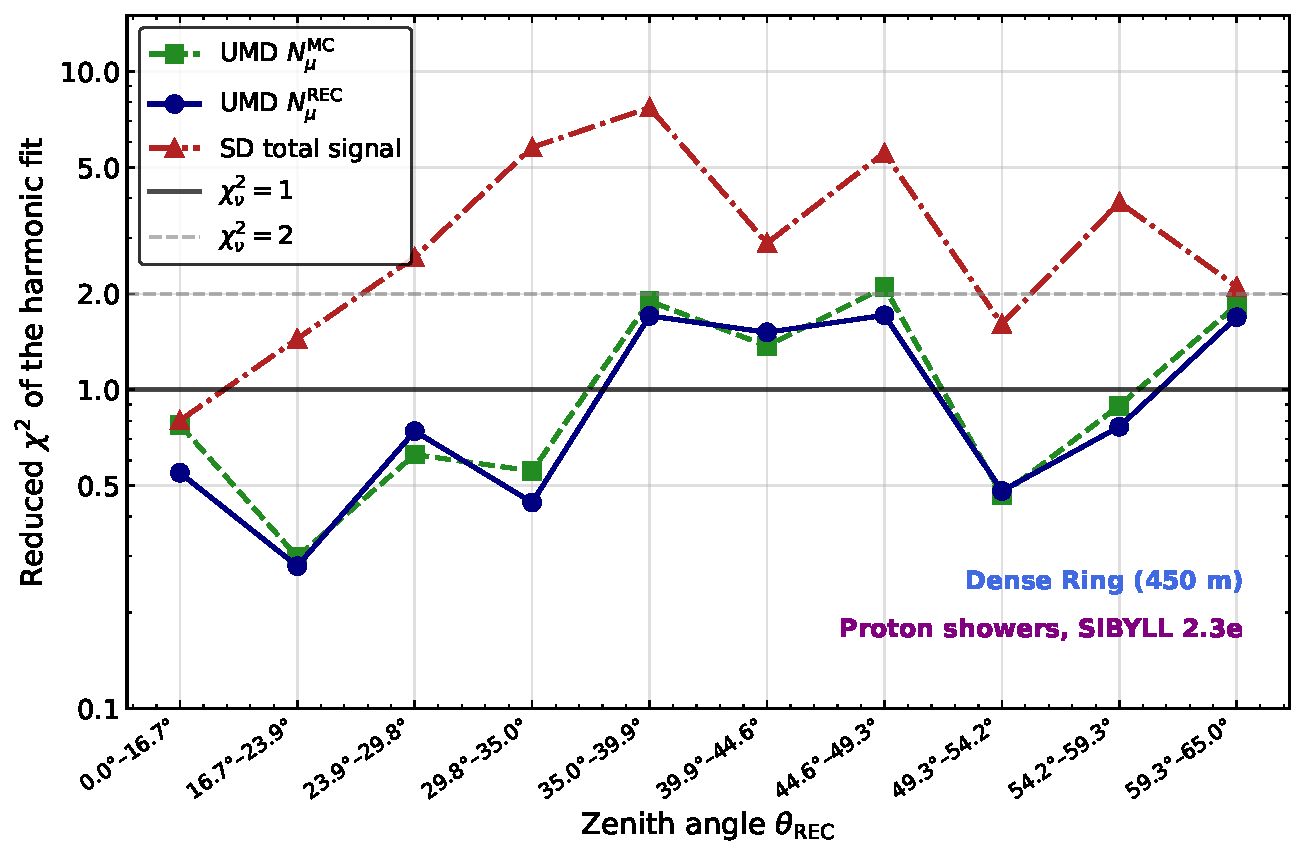
\includegraphics[width=\textwidth]{Backup_Chi2_DenseRing_EN.pdf}
    \column{0.37\textwidth}
      \begin{itemize}
        \item UMD, MC and REC: $\chi^2_\nu\approx1$ (0.3 to 2.1).
        \item SD: $\chi^2_\nu$ up to $\sim8$. With such small errors the fit is sensitive to
          higher harmonics and to correlations between stations of one shower.
      \end{itemize}
  \end{columns}
\end{frame}

\begin{frame}[t]{Backup: robustness}
  \badgeAD
  \vspace{-0.6em}
  \centering
  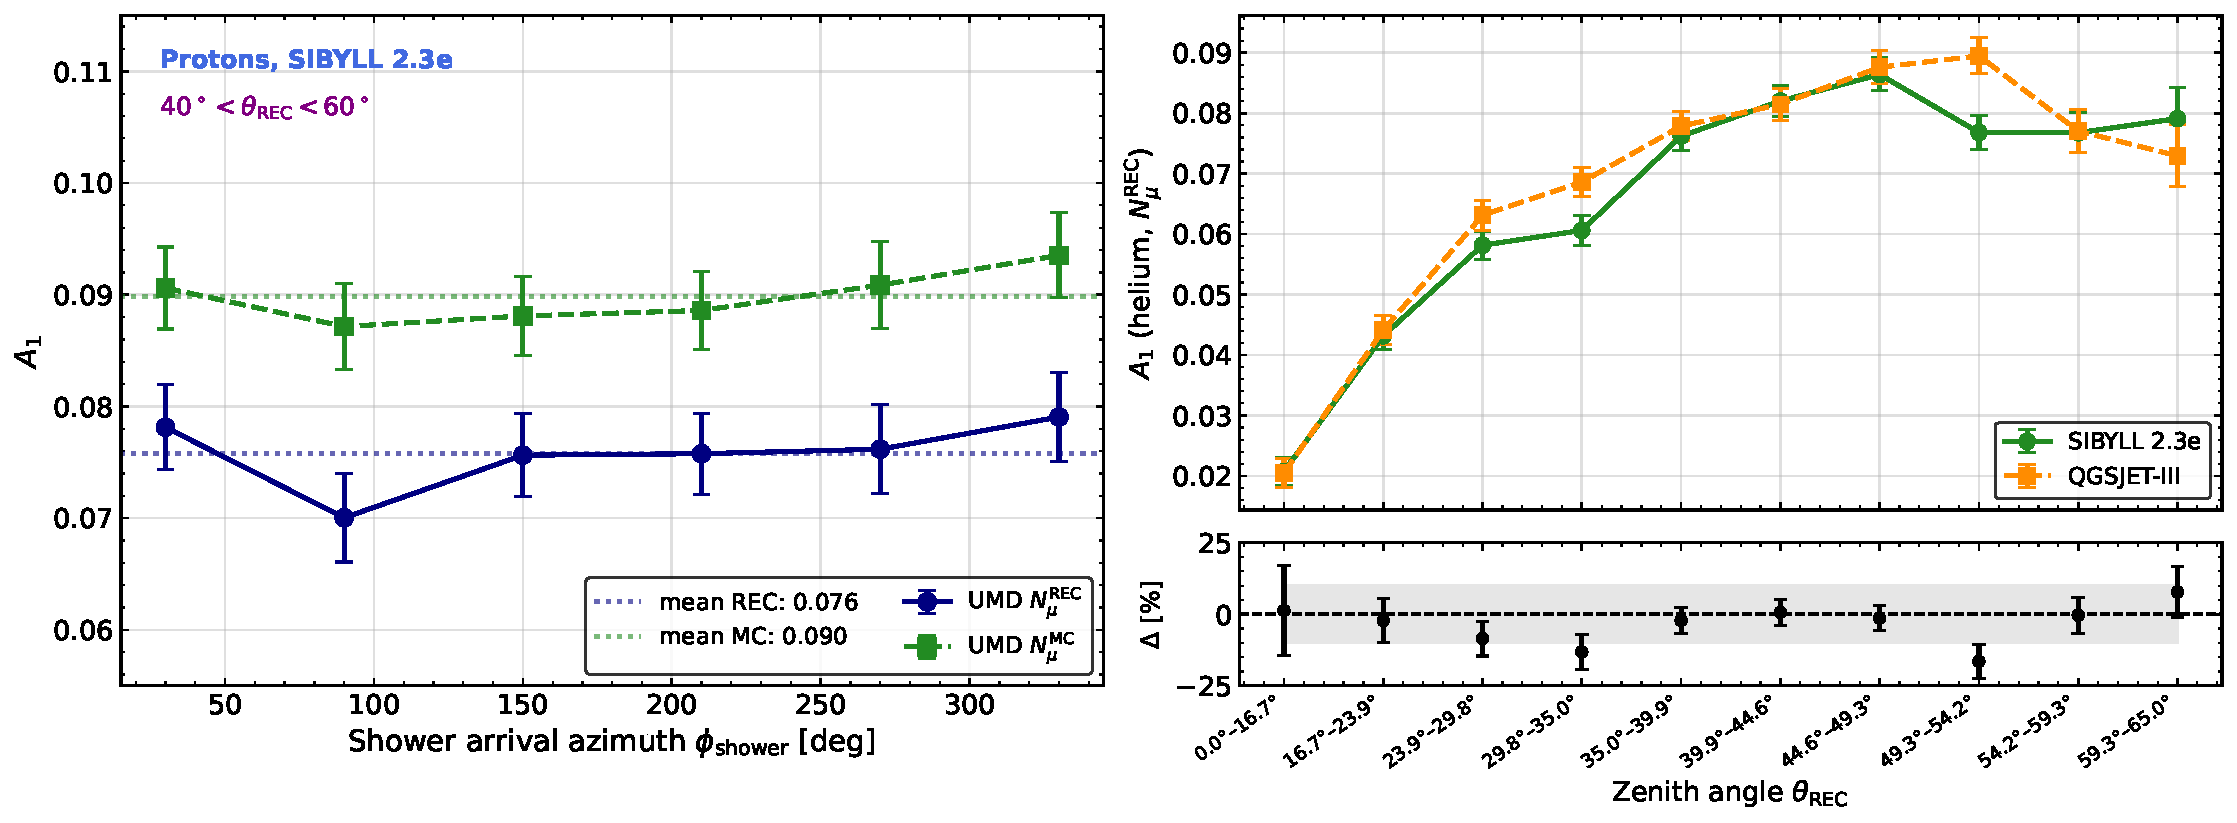
\includegraphics[width=\textwidth,height=5.1cm,keepaspectratio]{Backup_Robustness_EN.pdf}

  \raggedright
  \footnotesize
  \setbeamerfont{itemize/enumerate body}{size=\footnotesize}
  \begin{itemize}
    \setlength{\itemsep}{0pt}
    \item Left: $A_1$ does not depend on the arrival azimuth of the shower.
    \item Right: helium, SIBYLL~2.3e vs.\ QGSJET-III: within $\pm10\%$ over most of the range.
  \end{itemize}
\end{frame}

\begin{frame}{Backup: reconstruction performance}
  \centering
  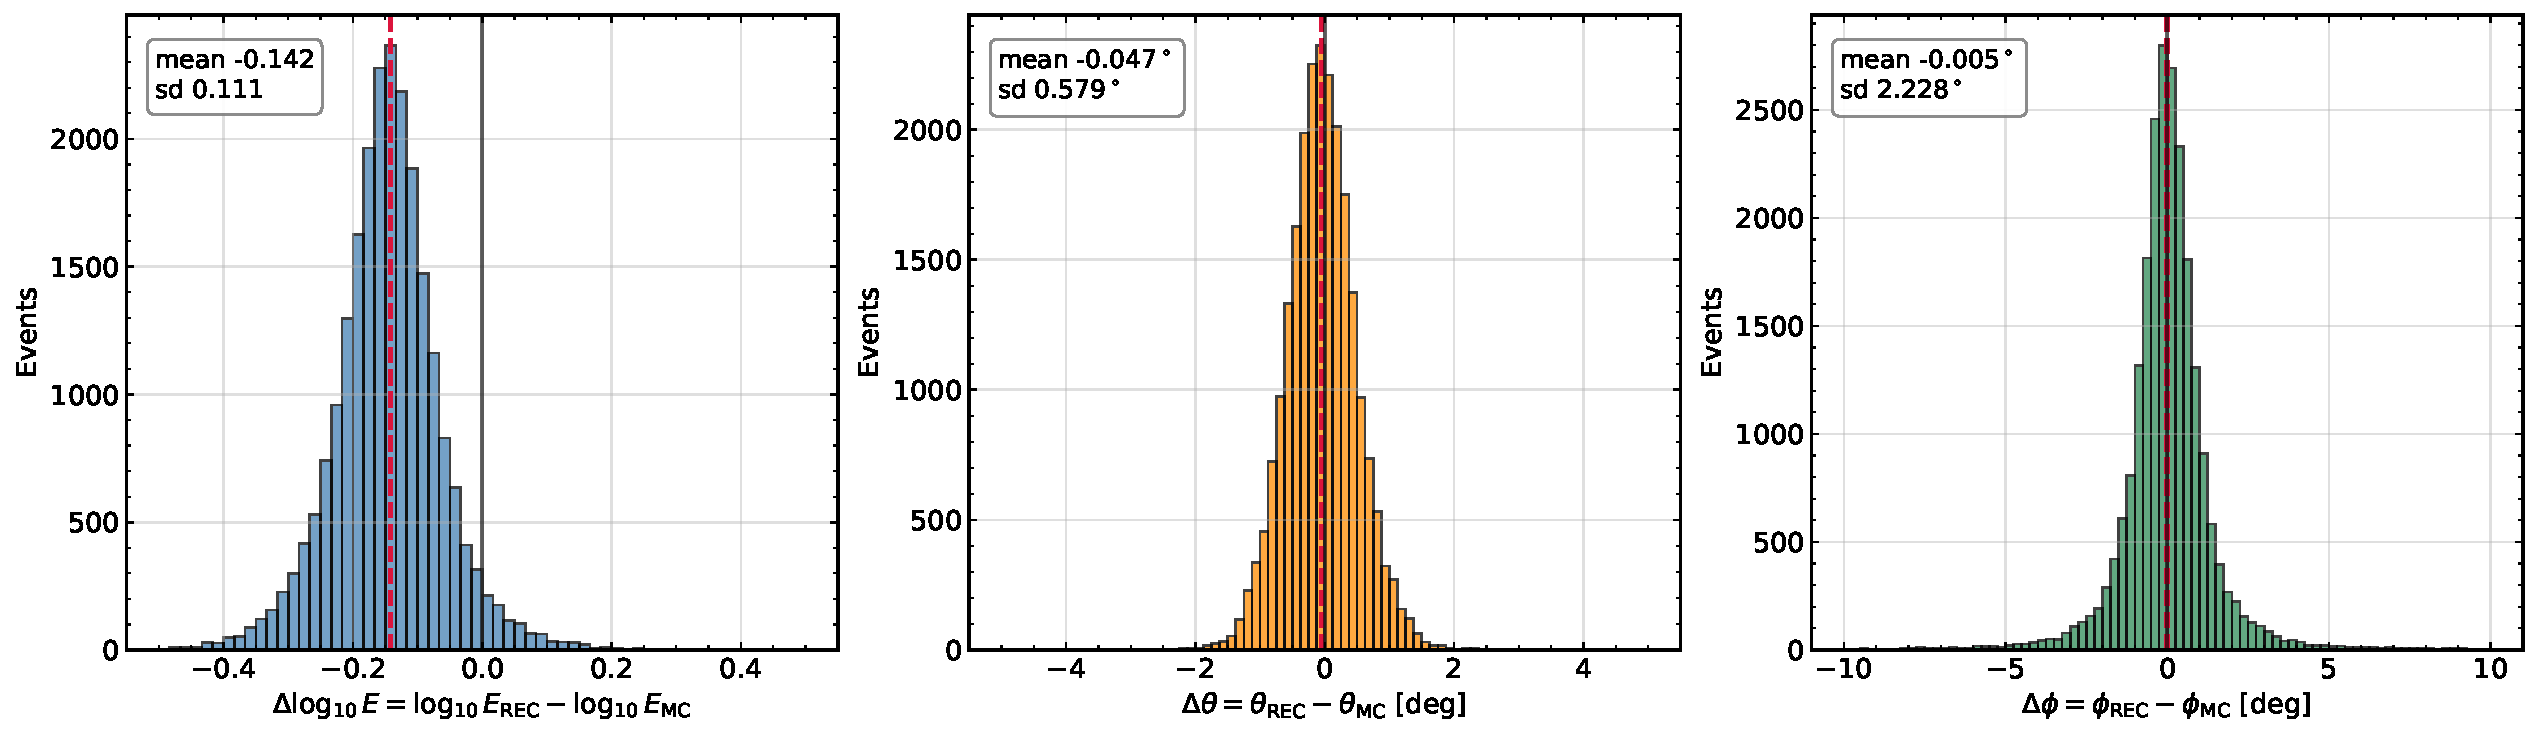
\includegraphics[width=\textwidth]{Backup_Reconstruction_EN.pdf}

  \raggedright
  \small
  \begin{itemize}
    \item Energy: mean $-0.142$, spread $0.111$ in $\Delta\log_{10}E$ (fewer muons in the
      simulation than in data, with a data-based energy calibration).
    \item $\theta$: bias $-0.05^\circ$, spread $0.58^\circ$. $\phi$: bias $-0.005^\circ$,
      spread $2.2^\circ$.
  \end{itemize}
\end{frame}

\begin{frame}{Backup: the core shift and the Dense Ring}
  \badgeAD
  \begin{itemize}
    \setlength{\itemsep}{0.5em}
    \item In reconstructed coordinates the ring \textbf{is} eccentric, but the stations are
      physically at 450~m from the \textbf{true} axis, and they are not re-binned in $r$.
    \item The assigned azimuth rotates by $\sim b/r\approx2^\circ$, much less than the
      $30^\circ$ spacing; the assigned radius changes by at most $b\approx20$~m.
    \item Both affect $N_\mu^{\text{MC}}$ and $N_\mu^{\text{REC}}$ in the same way, so they cannot
      explain the MC--REC gap on the ring (that gap is the counting bias).
  \end{itemize}
\end{frame}

\begin{frame}{Backup: is the UMD biased by the selection too?}
  \badgeIF
  \small
  \begin{itemize}
    \setlength{\itemsep}{0.4em}
    \item The UMD has no trigger of its own: a module is read only if the tank of its station
      is kept. So the UMD curve is also averaged over \texttt{HasStation} stations.
    \item But the selection acts on the \textbf{tank's own particles} (its muons and its EM
      signal). The module counts \textbf{other muons}: a different area, not right under the
      tank, behind $\sim$2.3~m of soil ($\sim$1~GeV threshold).
    \item Given the station position, the expected UMD count is still the local muon density:
      to first order, \textbf{no bias}.
    \item A residual effect can enter through what tank and module share, the fluctuation of
      the local density from shower to shower and station to station. Not quantified here; the
      UMD count of the stations that were not kept is not stored in this production.
  \end{itemize}
\end{frame}

\begin{frame}{Backup: SD muons over all stations vs.\ UMD}
  \badgeIF
  \vspace{-0.6em}
  \begin{columns}[c]
    \column{0.64\textwidth}
      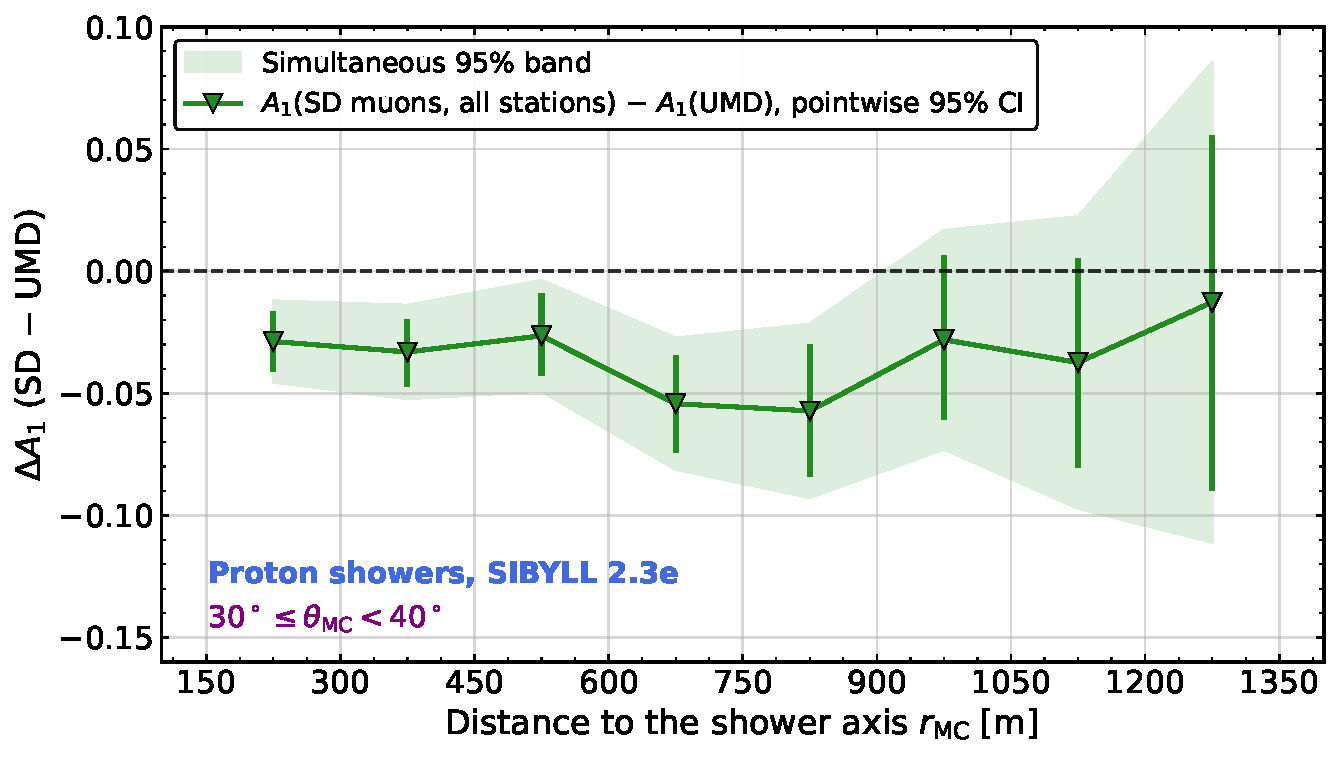
\includegraphics[width=\textwidth]{Selection_Difference_SD_UMD_EN.pdf}
    \column{0.34\textwidth}
      \footnotesize
      \setbeamerfont{itemize/enumerate body}{size=\footnotesize}
      \begin{itemize}
        \item Without \texttt{HasStation}, the SD muons stay \textbf{below} the UMD:
          $\Delta A_1\approx-0.03$ to $-0.06$ between 150 and 900~m.
        \item There the pointwise 95\% interval excludes zero; beyond 900~m the difference
          is not resolved.
        \item Paired bootstrap over the 960 showers (UMD and SD from the same showers).
        \item Candidates: flat plate vs.\ tank response, UMD threshold. Open.
      \end{itemize}
  \end{columns}
\end{frame}



\end{document}
